\documentclass[12pt, twoside, a4paper, xetex]{report}
%report中的chapter仅仅在新页开始,不强制在奇数页。
\usepackage{hcypaperstyle}

\begin{document}

\title{{\Huge 本科毕业设计论文\\}基于动态链接技术的web服务器动态扩展功能接口的设计与实现}
\author{黄丛宇\\06161032\\指导老师:马瑞芳}
\date{\today}

\maketitle

\lfour

\zhabstract 

Web服务器作为互联网的核心组成部分,在支撑整个互联网服务中,起到了至关重要的作用。由于互联网中应用的不断更新,要求web服务器也能适应这种更新变化。同时,web服务器必须保证7*24小时的运行。在目前的正在使用的web服务器中,大部分都不支持功能的动态增加,也就是在不重启服务器的情况下,动态的为服务器增加功能。针对这一问题,本课题基于动态链接库技术,使服务器在运行期间,可以动态的获知模块的增加并加载模块。本系统实现了服务器的基本功能,重点实现模块动态加载特性,并对实现进行测试。 

本论文的主要内容是研究实现基于动态链接技术的Web服务器动态加载插件的接口。首先,文中介绍了本课题的背景和意义,以及作者的主要任务和工作。接着概述与本课题相关的HTTP协议(RFC2616)的内容,简单介绍动态链接技术及其使用,还有介绍Web服务器的一些主流设计和实现方法。接下来,通过对HTTP协议的分析,设计插件的接口,分析动态链接技术,设计动态加载插件的过程。然后,采用非阻塞I/O+线程池+I/O多路复用技术,设计服务器的架构。然后,根据以上的设计,在Linux系统下,实现服务器的原型,并在其上实现插件接口和动态加载功能。

最后,通过测试和观察运行结果,分析服务器是否可以正确处理HTTP请求,包括HTTP/1.1的持久连接和HTTP/1.0的非持久连接,并返回客户端所请求的资源。同时,验证插件接口的设计能否满足扩展功能的需求,能否正确的动态加载插件。本系统可以处理一般规模的请求数量。

{\zhkeywords Web服务器;插件;Linux;C;动态加载}

\enabstract
I will translate it later...

{\enkeywords Web Server;Plugin;Linux;C;Dynamic load}

\newpage
\tableofcontents

\chapter{绪论}

\section{研究背景和意义}
\subsection{Web服务器的背景}
	Web服务器也称为WWW(Word Wide Web)服务器,主要功能是提供网上信息浏览服务。Web服务器通过解析处理HTTP协议完成客户端的请求。当Web服务器接收到一个HTTP请求时,通过解析请求的内容,经过一些列的处理(如,查找客户端请求的资源),生成一个HTTP响应并发送给客户端。这个HTTP响应包含客户端所请求的数据(例如送回一个HTML页面)或者提示信息等。在处理一个请求,Web服务器可以返回给客户端一个静态页面或图片,进行页面跳转,或者把动态响应委托给一些其它的程序处理(例如CGI脚本,JSP脚本,ASP脚本,或者一些其它的服务器端技术)。这些处理委托请求的服务器端程序通常产生一个HTML的响应,并通过web服务器发送给客户端。
	
	目前,主流的web服务器包括Apache,Lighttpd和Nginx。\ucite{baike}
	\begin{itemize}
		\item Apache是世界排名第一的web服务器,是Apache软件基金会的一个开放源码的web服务器。Apache可以运行在几乎所有的计算机平台上,如,Linux,Windows,Unix等。Apache快速、可靠并且可通过简单的API扩充。Apache web服务器具有如下特点:
		\begin{itemize}
			\item 支持通用网关接口和FastCGI
  			 \item 支持多种方式的HTTP认证
  			\item 支持实时监视服务器状态和定制服务器日志
  			\item 支持服务器端包含指令(SSI)
  			\item 支持安全Socket层(SSL)
  			\item 提供用户会话过程的跟踪
  			\item 通过第三方模块可以支持Java Servlets
		\end{itemize}
		\item Lighttpd是一个德国人领导的开源软件,根本在于提供一个专门针对高性能网站,安全、快速、兼容性好并且灵活的web服务器。Lighttpd具有非常低的内存开销,cpu占用率低,较好的性能以及丰富的模块。Lighttpd主要针对Unix/Linux平台,通过Cygwin也可以运行在Windows平台上,具有较好的夸平台特性。Lighttpd具有如下特性:
		\begin{itemize}
			\item 虚拟主机
  			\item virtual directory listings URL-Rewriting,HTTP-Redirects
  			\item automatic expiration offiles
  			\item 大文件支持(64bit file offsets)
  			\item 断点续传(start-end,start-,-end,multipleranges)
  			\item 压缩输出(支持deflate,gzip,bzip2)
  			\item CGI, FastCGI
		\end{itemize}
		\item Nignx("engine x")是一个高性能的HTTP和反向代理服务器,也是一个IMAP/POP3/SMTP代理服务器。 Nginx是由Igor Sysoev为俄罗斯访问量第二的Rambler.ru站点开发的,它已经在该站点运行超过两年半了。Igor将源代码以类BSD 许可证的形式发布。尽管还是测试版,但是Nginx已经因为它的稳定性、丰富的功能集、示例配置文件和低系统资源的消耗而闻名了。Nginx具有如下特点:
		\begin{itemize}
			\item 处理静态文件,索引文件以及自动索引
  			\item 反向代理加速(无缓存),简单的负载均衡和容错
  			\item FastCGI,简单的负载均衡和容错
  			\item 模块化的结构
  			\item SSL和TLS SNI支持
  			\item IMAP/POP3代理服务功能
  			\item 使用外部 HTTP认证服务器重定向用户到IMAP/POP3后端
  			\item 使用外部 HTTP认证服务器认证用户后连接重定向到内部的SMTP后端
		\end{itemize}
	\end{itemize}
	
	在这三个主流服务器的当前版本中,对于新的功能模块,都必须重启服务器才能是模块生效。然而有些时候,在怎加服务器功能的时候,不能对服务器进行重启,否则将会造成客户端当前状态的丢失,致使客户端当前正在进行的所有操作都将变的无效。比如,服务器和客户端保持了一个持久的连接,服务器不断的处理来自客户端的请求,而每个请求之间又保持着某种数据上的联系。也就是,前一个请求的处理结果影响下一个请求的处理结果。这时候,如果需要增加服务器的功能,同时增加的功能要立刻应用到当前的连接中,那么,服务器就不能进行重启。一旦服务器进行重启,由于HTTP协议不记录连接的状态,当前连接的所有状态都将丢失,那么,客户端的所有请求都将作废并重新开始。在一些场合,这将造成很严重的后果。
	
\subsection{动态链接技术背景}
	%程序员的自我休养---链接、装载和库 俞甲子 石凡 藩爱民 著 电子工业出版社
	动态链接技术是指,在程序的链接阶段,不对一些目标文件进行链接,等到程序运行时,再对这些目标文件进行链接的技术。也就是说,对于一些目标文件,把链接的过程推迟到了运行时在进行\ucite{cxyzwxy}。
	
	动态链接相对于静态链接有很多优点。对于静态链接,存在很严重的内存和磁盘空间的浪费,模块的更新也很困难。对于多个使用同一个库的程序,如果使用静态链接,那么每个程序的目标文件中都保存有这个库的一个副本。在程序运行的时候,每个程序在内存中也都有一个这个库的副本,这就对内存造成了很大的浪费。比如\ucite{cxyzwxy},在Linux系统中,一个普通的程序会使用到的C语言静态库至少在1MB以上,那么,如果在机器中有100个这样的程序,就要浪费掉近100MB的内存。如果磁盘中有2000个这样的程序,就要浪费近2GB的磁盘空间,很多Linux系统中,\verb|/usr/bin|下就有数千个可执行程序。另外,由于库是直接链接到程序的目标文件中的,一旦对库进行更新,将不会影响到程序中的副本,除非对程序进行重新编译。如果要对系统中所有使用这个库的程序进行重新编译,将是一个非常巨大的工作,很多情况下是不可能完成的(比如,没有程序的源文件)。比如,更新了Linux系统中的C语言静态库,那么就要对\verb|/usr/bin|下的那数千的程序进行重新链接。这将是一个繁重的工作。如果更新的是Windows系统中的库,由于很多程序无法获得源代码,也就无法进行重新链接,那么也就无法进行更新。
	
	动态链接则可以很好的解决上面的两个问题。当库是以动态链接的方式链接到程序中时,程序的目标文件中不包含有库的副本,仅仅是在调用库的地方做一个标记,同时在目标文件中记录所依赖的动态库。在程序运行时,操作系统从程序的目标文件中获知程序所依赖的动态库,然后在系统中查找这些动态库。接着,判断这些库是否已经加载到内存中,如果加载了,怎不需要在加载库,否则将库加载到内存中。如果有另一个程序需要同样的动态库,则不需要在将库加载到内存中,可以共享的使用内存中的副本。此时无论系统中运行了多少程序,所有的共享库在内存中只有一个副本,这就大大的提高了内存的使用效率。当需要对库进行升级的时候,仅仅需要将旧的库文件用新的覆盖掉,然后,重启系统中所有使用这个库的程序,那么所有程序都将使用新版的库。这就避免了对程序进行重新的链接。程序重启之后,库的更新工作急完成了。
	
	由于动态链接技术的这些特点,使得动态链接还具有另外一个特点:在程序运行时可以动态地选择加载各种程序模块。这个优点就可以用来制作程序的插件(Plug-in)。
	
\section{课题目标及作者的主要工作}
	本课题通过分析HTTP协议(RFC2616),设计插件所需的接口,通过使用动态链接技术,设计插件的动态加载的过程。最后,通过使用非阻塞I/O,I/O多路复用以及线程池的技术,构造出一个简单的Web服务器,并在这个服务器上验证插件接口的设计。最终,服务器将能完成基本的HTTP协议解析和处理,正确的加载和调用插件。
	
	\vspace{12pt}
	主要工作:
	\begin{enumerate}
		\item 学习动态链接库和web服务器设计实现的相关知识和技术                                
		\item 技术可行性论证,需求分析,构造系统结构                                            
		\item 搭建开发环境,编码实现 
		\item 测试插接接口的额可用性和服务器的性能                                                                                              
		\item 撰写毕业设计论文                                                                  
		\item 查找外文文献并翻译 
	\end{enumerate}
	
\section{论文章节结构}
	\subsection*{第一章是绪论,主要对本论文的主要内容进行了概述。}
	
	首先介绍了Web服务器和动态链接技术的背景。列举出当前主流的三个Web服务器(apache,lighttpd,nignx)的主要特定。在这些服务器的当前版本中,都不支持功能模块的动态加载。在加载模块时都要对服务器进行重启。
	
	下面是课题的主要目标和作者的主要工作。一方面描述了动态加载插件的接口的设计和实现的主要目标和服务器实现的目标,另一方面给出了作者在课题的进行期间的主要工作。
	最后,给出了本文的章节安排。
	
	\subsection*{第二章是服务器设计和实现技术,主要介绍当前主流的服务器的设计和实现技术}
		首先介绍了动态链接技术在主流平台上的实现,然后,通过一个在Linux平台上的小例子,讲解动态链接技术的使用,包括动态库的创建和使用。接下来介绍了有关非阻塞I/O和I/O多路复用的特点,阐述了在Linux平台下这两项技术的使用方法和注意事项,同时介绍了Linux平台下几种主流的I/O多路复用技术。下面介绍了线程池的设计和使用,以及线程池的优点。最后,介绍了状态机的一些基本知识。
		
	\subsection*{第三章是插件接口和服务器的分析和设计。包括分析RFC2616,根据HTTP协议设计接口,使用主流技术设计服务器。}
		首先是对HTTP协议(RFC2616)进行分析,包括HTTP协议的处理过程和数据格式。在对HTTP协议分析的基础上,设计插件的接口以及接口在处理HTTP协议时调用的过程。基于动态链接技术,设计模块的动态加载的过程,并给出设计方案。
		然后,介绍了服务器的I/O设计,通过使用非阻塞I/O和I/O多路复用来提高服务器的I/O效率。同时,基于线程池,对I/O事件进行多线程并行化处理,进一步提高效率。接着,基于状态机技术,将一个连接的不同时段标记成不同的状态,通过状态机对连接的生命周期进行管理。
	
	\subsection*{第四章是插件接口和服务器的实现和测试。主要是在Linux平台下实现插件接口和服务器,并对其进行测试}
		首先是插件接口的实现,通过使用C语言的结构体,将每个插件与一个结构体对应,来实现对插件的管理和调用,插件的接口被实现为一些列标准的函数。接着是介绍动态加载过程的实现,主要是基于Linux平台上的Inotify技术,实现动态加载。然后,实现插件在处理HTTP协议时的调用过程。下面是服务器的I/O实现,主要使用Linux平台中的epoll来完成I/O事件监测。接着,利用Linux下的Pthread实现线程池。然后实现处理连接状态的状态机。
		最后,通过对系统的测试。包括功能测试和性能测试。功能测试主要测试系统能否完成预定的功能,包括HTTP协议处理和插件动态加载和调用。性能测试包括测试服务器的性能,找出性能瓶颈并给出可能的解决方案。
	\subsection*{第五章为结束语。包括整篇论文的总结和对Web服务器设计的未来的展望}
		首先总结了本人在整个毕业设计期间的工作以及经验和教训。
		然后是展望,对Web服务器领域的前景做出展望,提出课题中所设计的服务器的不足和改进。
	
\chapter{服务器设计和实现技术}

\section{HTTP协议}
	HTTP协议(Hypertext Transfer Protocol,超文本传输协议)是一个属于应用层的面向对象的协议。它于1990年提出。主要用于从WWW服务器传输超文本到本地浏览器的传送协议。
	
	HTTP是一个客户端和服务器端请求和应答的标准。客户端是终端用户,服务器端是网站。通过使用Web浏览器、网络爬虫或者其它的工具,客户端发起一个到服务器上指定端口(默认端口为80)的HTTP请求。应答的服务器上存储着(一些)资源,比如HTML文件和图像。我们称这个应答服务器为源服务器(origin server)。\ucite{wiki}
	
	通常,由HTTP客户端发起一个请求,建立一个到服务器指定端口(默认是80端口)的TCP连接。HTTP服务器则在那个端口监听客户端发送过来的请求。一旦收到请求,服务器(向客户端)发回一个状态行,比如"HTTP/1.1 200 OK",和(响应的)消息,消息的消息体可能是请求的文件、错误消息、或者其它一些信息。通过HTTP或者HTTPS协议请求的资源由统一资源标识符(Uniform Resource Identifiers,URI)来标识。
	
	HTTP/1.1协议中共定义了八种方法(有时也叫“动作”)来表明Request-URI指定的资源的不同操作方式\ucite{wiki}:
	\begin{enumerate}
		\item OPTIONS 返回服务器针对特定资源所支持的HTTP请求方法。也可以利用向Web 服务器发送'*'的请求来测试服务器的功能性。
		\item HEAD 向服务器索要与GET请求相一致的响应,只不过响应体将不会被返回。这一方法可以在不必传输整个响应内容的情况下,
					就可以获取包含在响应消息头中的元信息。
		\item GET 向特定的资源发出请求。注意:GET方法不应当被用于产生“副作用”的操作中,例如在Web Application中。
					其中一个原因是GET可能会被网络蜘蛛等随意访问。参见安全方法
		\item POST 向指定资源提交数据进行处理请求(例如提交表单或者上传文件)。数据被包含在请求体中。POST请求可能会导致新的资源的建立和/或已有资源的修改。
		\item PUT 向指定资源位置上传其最新内容。
		\item DELETE 请求服务器删除Request-URI所标识的资源。
		\item TRACE 回显服务器收到的请求,主要用于测试或诊断。
		\item CONNECT HTTP/1.1协议中预留给能够将连接改为管道方式的代理服务器。
	\end{enumerate}
	
	HTTP服务器至少应该实现GET和HEAD方法,其他方法都是可选的。当然,所有的方法支持的实现都应当符合下述的方法各自的语义定义。此外,除了上述方法,特定的HTTP服务器还能够扩展自定义的方法。
	
	所有HTTP响应的第一行都是状态行,依次是当前HTTP版本号,3位数字组成的状态代码,以及描述状态的短语,彼此由空格分隔。状态代码的第一个数字代表当前响应的类型\ucite{wiki}:
	\begin{itemize}
		\item 1xx 消息——请求已被服务器接收,继续处理
		\item 2xx 成功——请求已成功被服务器接收、理解、并接受
		\item 3xx 重定向——需要后续操作才能完成这一请求
		\item 4xx 请求错误——请求含有词法错误或者无法被执行
		\item 5xx 服务器错误——服务器在处理某个正确请求时发生错误
	\end{itemize}
	
	HTTP协议已经演化出了很多版本,它们中的大部分都是向下兼容的。在RFC 2145中描述了HTTP版本号的用法。客户端在请求的开始告诉服务器它采用的协议版本号,而后者则在响应中采用相同或者更早的协议版本。
	\begin{itemize}
		\item 0.9 已过时。只接受GET一种请求方法,没有在通讯中指定版本号,且不支持请求头。由于该版本不支持POST方法,因此客户端无法向服务器传递太多信息。
		\item HTTP/1.0 这是第一个在通讯中指定版本号的HTTP协议版本,至今仍被广泛采用,特别是在代理服务器中。
		\item HTTP/1.1 当前版本。持久连接被默认采用,并能很好地配合代理服务器工作。还支持以管道方式在同时发送多个请求,以便降低线路负载,提高传输速度。
	\end{itemize}
	%http://zh.wikipedia.org/zh-cn/%E8%B6%85%E6%96%87%E6%9C%AC%E4%BC%A0%E8%BE%93%E5%8D%8F%E8%AE%AE
\section{动态链接技术}
	\subsection{动态链接的实现}
	动态链接设计运行时的链接及多个文件的加载,必须要有操作系统的支持,因为动态链接的情况下,进程的虚拟地址空间的分部会比静态链接情况下更为复杂。目前主流的操组系统的几乎都支持动态链接这种方式,在Linux系统中,ELF动态链接文件被称为动态共享对像(DSO,Dynamic Shared Objects),简称共享对象,他们一般是以“.so”为扩展名的一些文件。在Window系统中,动态链接文件被称为动态链接库(DLL, Dynamicla Linking Library),它们通常是我们平时很常见的".dll"为扩展名的文件。
	
	在程序被加载时,系统的动态链接器会将程序所需要的所有动态链接库装载到进程的地址空间中,并且程序中所有未决议的符号绑定到响应的动态链接库中,并进行重定位工作。动态链接把链接这个过程从程序加载前推迟到程序加载时,这会造成程序性能上的一些损失。据估算,动态链接与静态链接相比,性能损失大约在5\%以下。
	
	\subsection{动态库的创建和使用}
	在Linux下和Window下,动态库的创建和使用是不相同的。由于本课题主要是在Linux系统中进行,因此在这里,将通过一个例子来简单的介绍在Linux下动态库的使用\ucite{cxyzwxy}。例子的程序源码如下:
	
	\begin{verbatim}
	/* Program1.c*/
	#include "Lib.h"
	int main(int argc, char *argv[])
	{
		foobar(1);
		return 0;
	}
	
	/*Program2.c*/
	#include "Lib.h"
	int main(int argc, char *argv[])
	{
		foobar(2);
		return 0;
	}
	
	/*Lib.c*/
	#include <stdio.h>
	void foobar(int i)
	{
		printf("Printing from Lib.so %d\n", i);
	}
	/*Lib.h*/
	#ifndef LIB_H
	#define LIB_H
	void foobar(int i);
	#endif
	\end{verbatim}
	
	程序很简单,两个程序的主要模块Program1.c和Program2.c分别调用Lib.c里面的foobar()函数。
	在Linux下,我们使用gcc讲Lib.c编译成一个共享库:
	\begin{verbatim}
	gcc -fPIC -shared -o Lib.so Lib.c
	\end{verbatim}
	-fPIC和-shared是GCC的参数,这也是创建共享库的关键参数:
	\begin{itemize}
		\item -fPIC 表示使用地址无关代码(Position Independent Code)技术来产生输出文件。
		\item -shared 表示输出结果是共享库类型。
	\end{itemize}
	
	这时候,我们得到了一个Lib.so文件,这就是包含了Lib.c的foobar()函数的共享对象文件。然后,我们分别编译链接Program1.c和Program2.c:
	\begin{verbatim}
	gcc -o Program1 Program1.c ./Lib.so
	gcc -o Program2 Program2.c ./Lib.so
	\end{verbatim}
	
	从Program1的角度看,整个编译和链接的过程如图\ref{solink}
	\begin{figure}[htbp]
	\centering
	\setlength{\abovecaptionskip}{0pt}
	\setlength{\belowcaptionskip}{10pt}
	\caption{动态链接过程}
	\label{solink}
	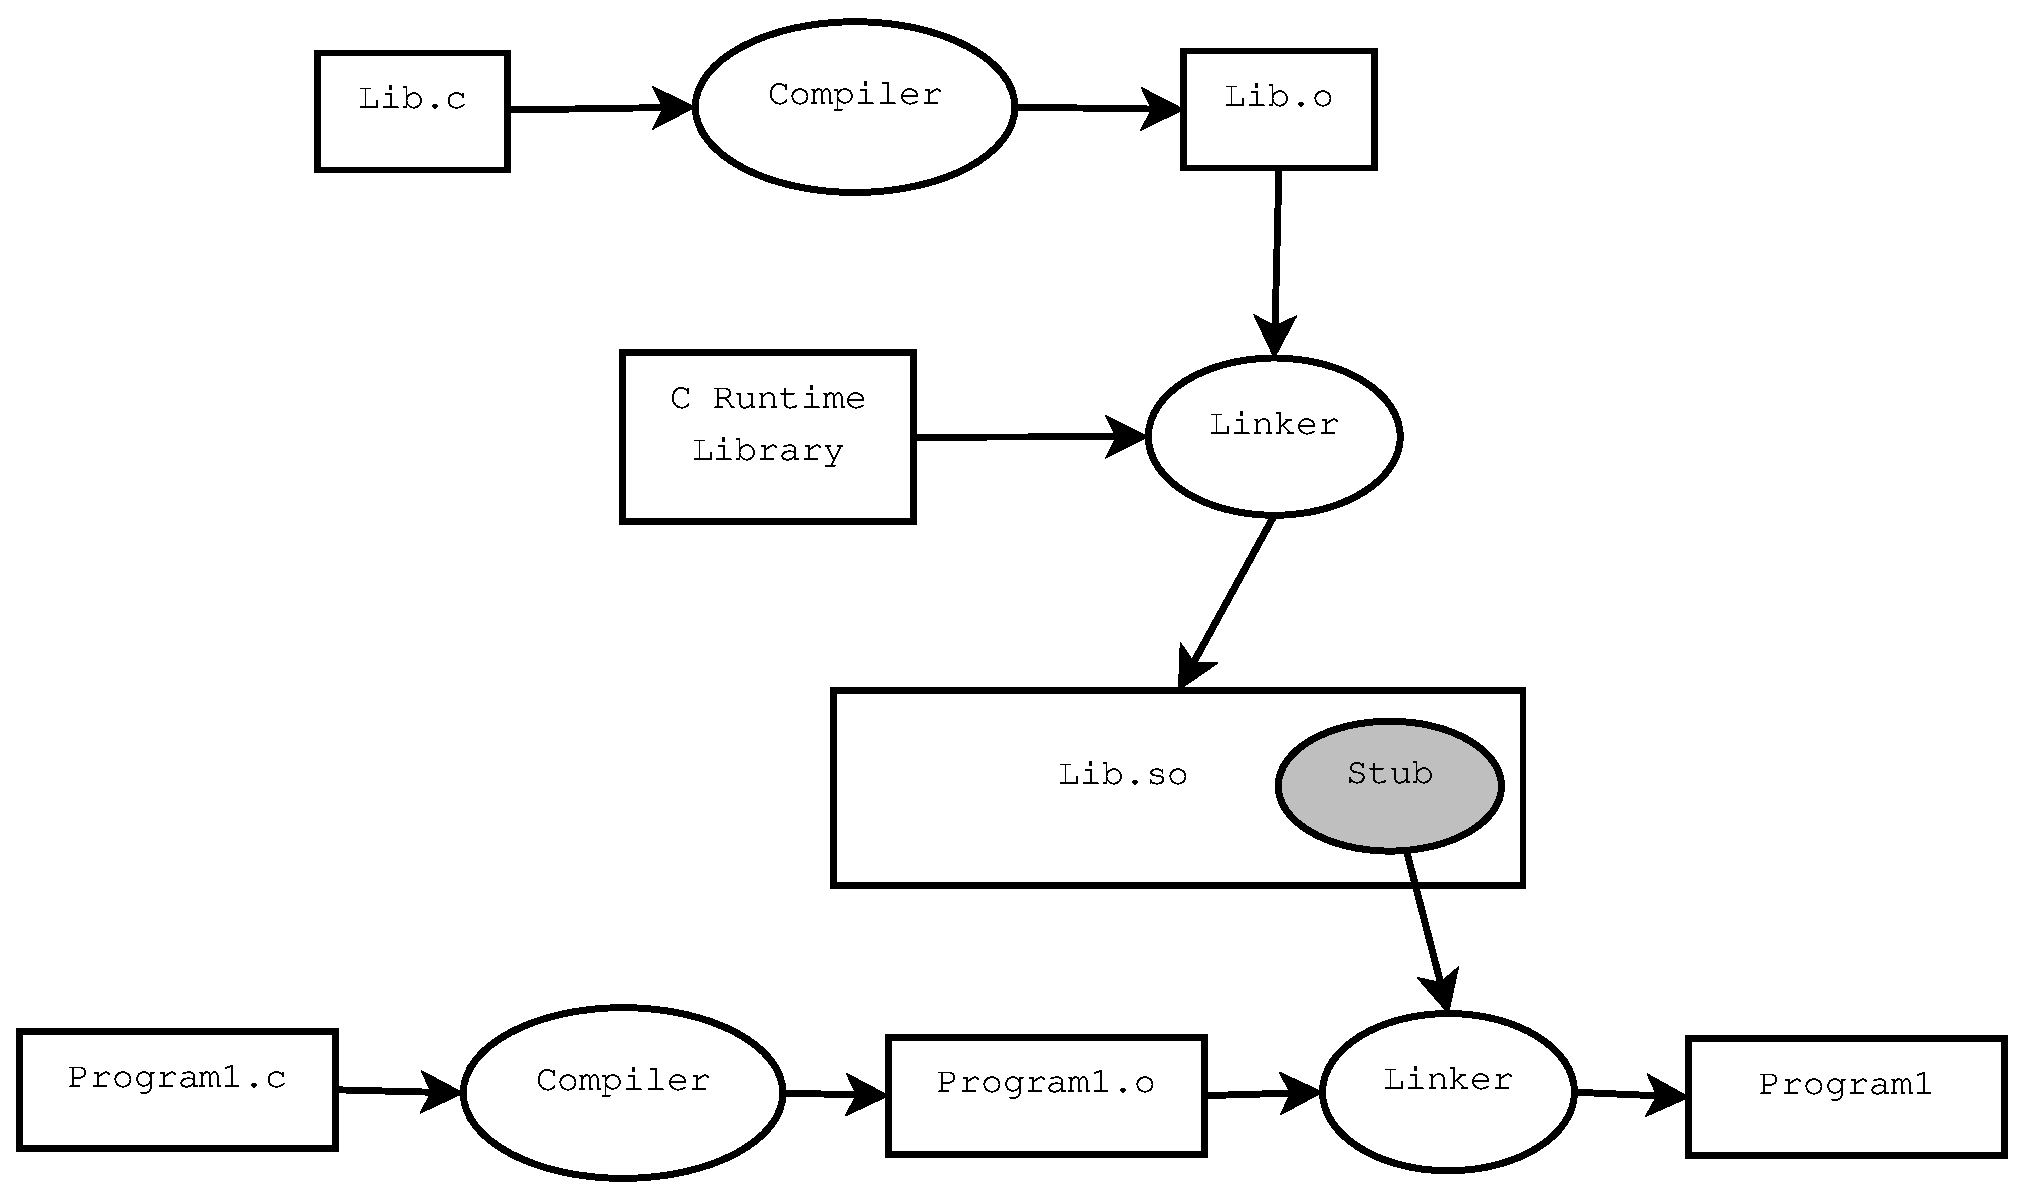
\includegraphics[height=9cm, width=15cm]{pics/solink.eps}
	\end{figure}
	
	在链接程序Program1时,没有将动态库链接到程序的目标文件中,而仅仅是做了一个标记。当系统加载程序Program1时,动态链接加载器会根据Program1目标文件中的信息,搜索共享库Lib.so并加载到内存中。完成最后的链接工作。
	
\section{非阻塞I/O与I/O多路复用}
	非阻塞I/O使我们可以调用open、read和write这样的I/O操作,并使这些操作不会永远阻塞。如果这种操作不能完成,则调用立即出错返回,表示该操作如继续执行将阻塞。\ucite{apue}
	
	对于一个给定的描述符有两种方法对其置顶非阻塞I/O:
	\begin{enumerate}
		\item 如果调用open获得描述符,则可指定O\_NONBLOCK标志。
		\item 对于已经打开的描述符,则可调用fcntl,有该函数打开O\_NONBLOCK文件状态标志。
	\end{enumerate}
	
	I/O多路复用(或者I/O夺路转接,I/O multiplexing),是指先构造一张有关描述符的列表,然后调用一个函数,知道这些描述符中的一个或多个已准备好进行I/O时,该函数返回,在返回时,它告诉进程那些描述符已经准备好进行I/O。\ucite{apue}
	
	I/O夺路服用有多种实现。主要包括:
	\begin{enumerate}
		\item 传统的select 对所监听的描述符数量有一个硬性的限制:FD\_SETSIZE。这个限制通常很难改变。另外,随着所监听的描述符的数量的增加,select的效率有明显的下降。这是由于select要对所有被监听的描述符进行扫描。
		\item 传统的poll 对监听的描述符数量没有硬性的限制。真正的显示通常来自机器的内存大小等。和select一样, 随着描述符的增加效率明显降低。
		\item /dev/poll 是Solaris中poll的替代品。
		\item kqueue 是FreeBSD中的poll的替代品。(也是NetBSD的)
		\item epoll 在Linux 2.6内核中被引入。是epoll的替代品。对描述符的数量没有限制(限制通常来自内存大小),并且,效率不随描述符数量的增加而下降。
		\item Completion Port NT内核(Window平台)中I/O多路复用的实现。
	\end{enumerate}
	
	图\ref{epollvspoll}是有关epoll和poll的效率比较。sys\_epoll和/dev/epoll是epoll的不同接口。
	\begin{figure}[htbp]
	\centering
	\caption{epoll与poll效率比较\ucite{hudong}}
	\label{epollvspoll}
	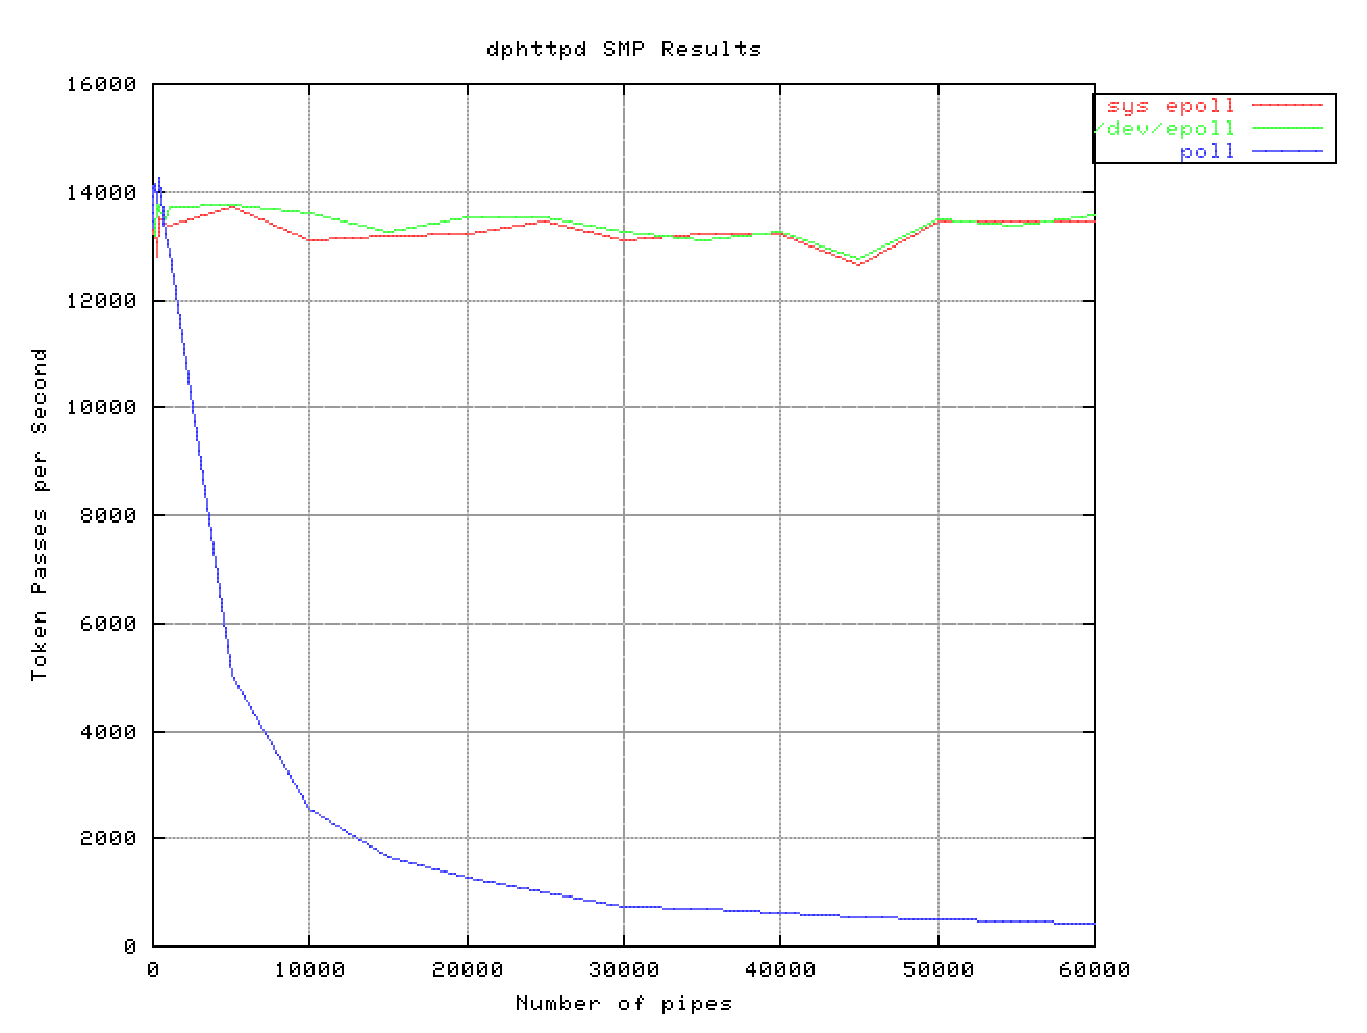
\includegraphics[height=11cm, width=15cm]{pics/epollvspoll.eps}
	\end{figure}
	
	由于本课题主要是在Linux平台下进行,因此,系统中使用Linux下推荐的epoll。
	
	epoll主要有三个接口函数:epoll\_create, epoll\_wait, epoll\_ctl。
	\begin{enumerate}
		\item epoll\_create 创建一个epoll实例,并返回一个epoll的描述符。这个描述符是后面两个函数的参数。
		\item epoll\_wait 等待epoll实例所监听的描述符发生I/O事件。一旦有描述符发生事件,返回这些描述符和对应的事件。
		\item epoll\_ctl 增加或删除epoll实例所监听的描述符,或修改描述符所监听的事件。
	\end{enumerate}
	
	epoll有两种模式:水平触发(level-triggered)和边际触发(edge-triggered)。当在水平触发模式时,只要有描述符处于就绪状态(比如,有数据可读),那么调用epoll\_wait时,epoll\_wait立即返回描述符及其对应事件。而当处于边际触发时,当有描述符从不就绪变成就绪,epoll\_wait返回描述符及其事件,并且epoll假设调用这已经知道了事件的发生并且会进行正确的处理。之后,无论多少次调用epoll\_wait,只要描述符的状态不发生变化(从不就绪变成就绪),就算此时有数据可以读,epoll都不会再次提醒调用者。这就有可能造成数据丢失。
	epoll默认处在水平触发模式。
	
\section{线程池}
	虽然线程的创建和初始化相对于进程来说,已经很快速了。但是,在很多程序中,特别是负载较高的服务器程序,频繁的创建销毁线程也会影响程序的运行效率。而线程池则可以避免掉对线程的频繁的创建和销毁。
	
	在线程池中通常会有若干个处于等待状态的线程。这些线程仅仅是处于等待状态,各种资源都是已经分配好的。当需要线程来处理某一个任务时,通过线程池获得一个处于等待状态的线程,然后通知这个线程去处理这个任务。此时的线程可以立即执行任务(准确的说是立即处于就绪状态),而不需要花费时间进行初始化等工作。当处理完任务后,线程重新回到线程池中,继续处于等待状态,直到下次任务到达。
	
	线程池中关键的是如何通知处于等待状态的线程有新的任务需要处理。这需要对应平台的线程库予以支持。在Linux下,线程的使用通常依赖pthread库。pthread库提供了一套线程的创建管理方法。其中,条件变量可以很好的实现通知等待线程的功能。条件变量是指线程等待某一事件的发生,在事件发生之前,线程一直处于等待状态。

\section{状态机}
	状态机,即有限状态机(Finite State Machine)。是表示有限个状态以及在这些状态之间的转移和动作等行为的数学模型\ucite{wiki}。
	
	图\ref{fsm}是一个简单的关于开门和关门的状态机。
	
	\begin{figure}[bp]
	\centering
	\caption{开门关门状态机\ucite{wiki}}
	\label{fsm}
	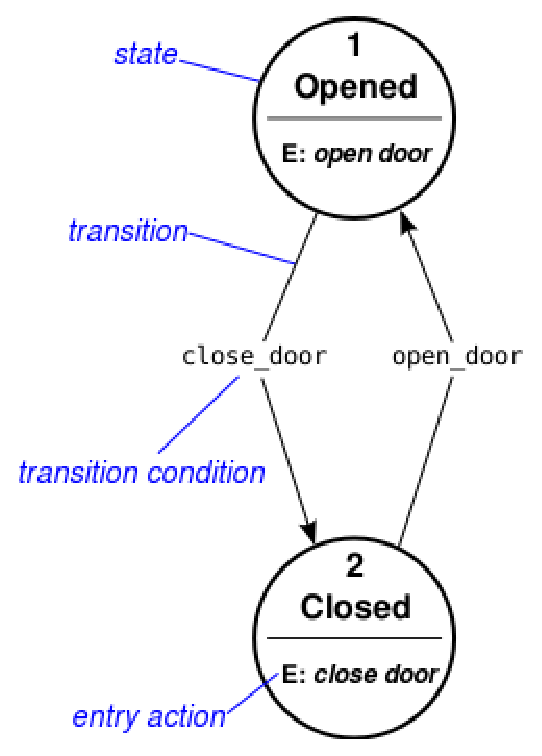
\includegraphics[height=8cm, width=6cm]{pics/fsm.eps}
	\end{figure}
	
	状态机可分为确定型(DFA)和非确定型(NDFA、GNFA)状态机。在确定型状态机中,每个状态对每个可能输入只有精确的一个转移。在非确定型状态中,给定状态对给定可能输入可以没有或有多于一个转移。
	
\chapter{插件接口和服务器的分析和设计}

\section{HTTP协议分析}
\subsection{HTTP协议的数据格式}
	HTTP协议的主要数据格式包括Request格式和Response格式。
	
	Request是客户端发送个服务器的请求数据。包括服务器完成请求所需要的信息。HTTP协议规定Request的格式如下:
\begin{verbatim}
    ---------------------------------------
    | Methods |sp| URI |sp| Version |cr|lf|  -----> Request line
    ---------------------------------------
    | Header Field Name: |sp| Value |cr|lf|  -]
    ---------------------------------------   |
    |   ... (more headers)                |   |---> Header lines
    ---------------------------------------   |
    | Header Field Name: |sp| Value |cr|lf|  -]
    ---------------------------------------
    |cr|lf|                                  -----> a blank line
    ---------------------------------------
    |                                     |
    | Data...                             |  -----> Entity body
    |                                     |
    ---------------------------------------
      cr = \r ; lf = \n ; sp = blankspace
\end{verbatim}
 	
 	从上面的格式可以看出,Request的格式非常简单,包括Request line,Header lines和 Entity body三个部分。Request line包含请求的方法,请求资源的URI以及客户端所使用的HTTP协议的版本。其中,对于所请求的资源的URI中的特殊字符(如汉字),客户端要对其进行编码。编码的格式为“\% HEX HEX”(具体参见RFC 2396)。Header lines包含一些“key:value”形式的键值信息,是客户端发送给服务器的有关自身信息或者链接处理方式等数据。这些键值信息的键在HTTP协议中有明确的规定,服务器一般不对这些键值信息的意义进行更改或扩充HTTP协议规定之外的键值信息。Entity body中包含客户端发送给服务器的数据。这些数据通常对服务器透明,也就是说服务器不需要关心这些数据的意义,只需要将这些数据传递给一些处理链接请求的委托程序(如,CGI脚本),由这些委托程序进行处理。在HTTP协议中,没有对Entity body中的数据的格式和意义做任何形式的规定或定义。
 	
 	Response的格式与Request格式类似。Response数据由服务器处理完请求之后,发送给客户端。Response格式如下:
\begin{verbatim}
-----------------------------------------------
|Version|sp|Status-Code|sp|Reason-Phrase|cr|lf| ---> Status line
-----------------------------------------------
| Header Field Name:   |sp|  Value      |cr|lf| -]
-----------------------------------------------  |
|  ... (more headers)                         |  |-> Header lines
-----------------------------------------------  |
| Header Field Name:   |sp|    Value    |cr|lf| -]
-----------------------------------------------
|cr|lf|                                        ---> a blank line
-----------------------------------------------
|                                             |
| Data...                                     |  ---> Entity body
|                                             |
-----------------------------------------------
 cr = \r ; lf = \n ; sp = blankspace
\end{verbatim}

 	Response格式和Resquest格式的主要区别在第一行的Status line。Status line包含HTTP 协议的版本,请求处理结果的状态码和结果原因描述。Response中Header lines中的键值对和Request中的键值对一样,都是由HTTP协议进行明确的规定。Entity body包含处理结果。
 	
\subsection{HTTP协议的处理过程}
	通常,在HTTP协议中,有客户端发起请求,服务器被动的接受请求。如图\ref{httpbaike}
	\begin{figure}[htbp]
	\centering
	\caption{HTTP协议的处理过程\ucite{baike}}
	\label{httpbaike}
	
\includegraphics[height=3cm, width=8cm]{pics/httpbaike.eps}
	\end{figure}
	
	在客户端和服务器之间建立连接之后,客户端发送Request数据,服务器对Request数据进行解析然后按照解析出来的数据对请求进行处理,处理完毕之后(包括处理出错),服务器构造Response数据,返回给客户端。在整个过程中,服务器对客户端的请求不做任何信息或者状态的记录。也就是说,即使是同一客户端的同一个请求,多次发送给服务器,服务器都认为是不同的请求。在本课题中,我们主要关心在服务器端HTTP协议的处理过程。如图\ref{serverhttp}。
	\begin{figure}[htbp]
	\centering
	\caption{服务器端HTTP协议的处理过程}
	\label{serverhttp}
	\includegraphics[height=8cm, width=10cm]{pics/serverhttp.eps}
	\end{figure}
	
\section{插件接口的分析和设计}
\subsection{插件调用过程的分析和设计}
	在图\ref{serverhttp}中可以看到,服务器在处理HTTP请求的时候,基本上分为三步:解析协议,处理请求和返回处理结果。在解析协议和返回处理结果的过程中,服务器都要必须严格按照HTTP协议的规定进行处理,这两个过程中,没有必要也不能增加HTTP协议规定之外的处理步骤。并且,插件基本上都是针对处理请求设计的,因此,插件的调用过程集中在处理请求的阶段。插件的调用过程如图\ref{httpplugin}所示。
	\begin{figure}[htbp]
	\centering
	\caption{插件调用过程}
	\label{httpplugin}
	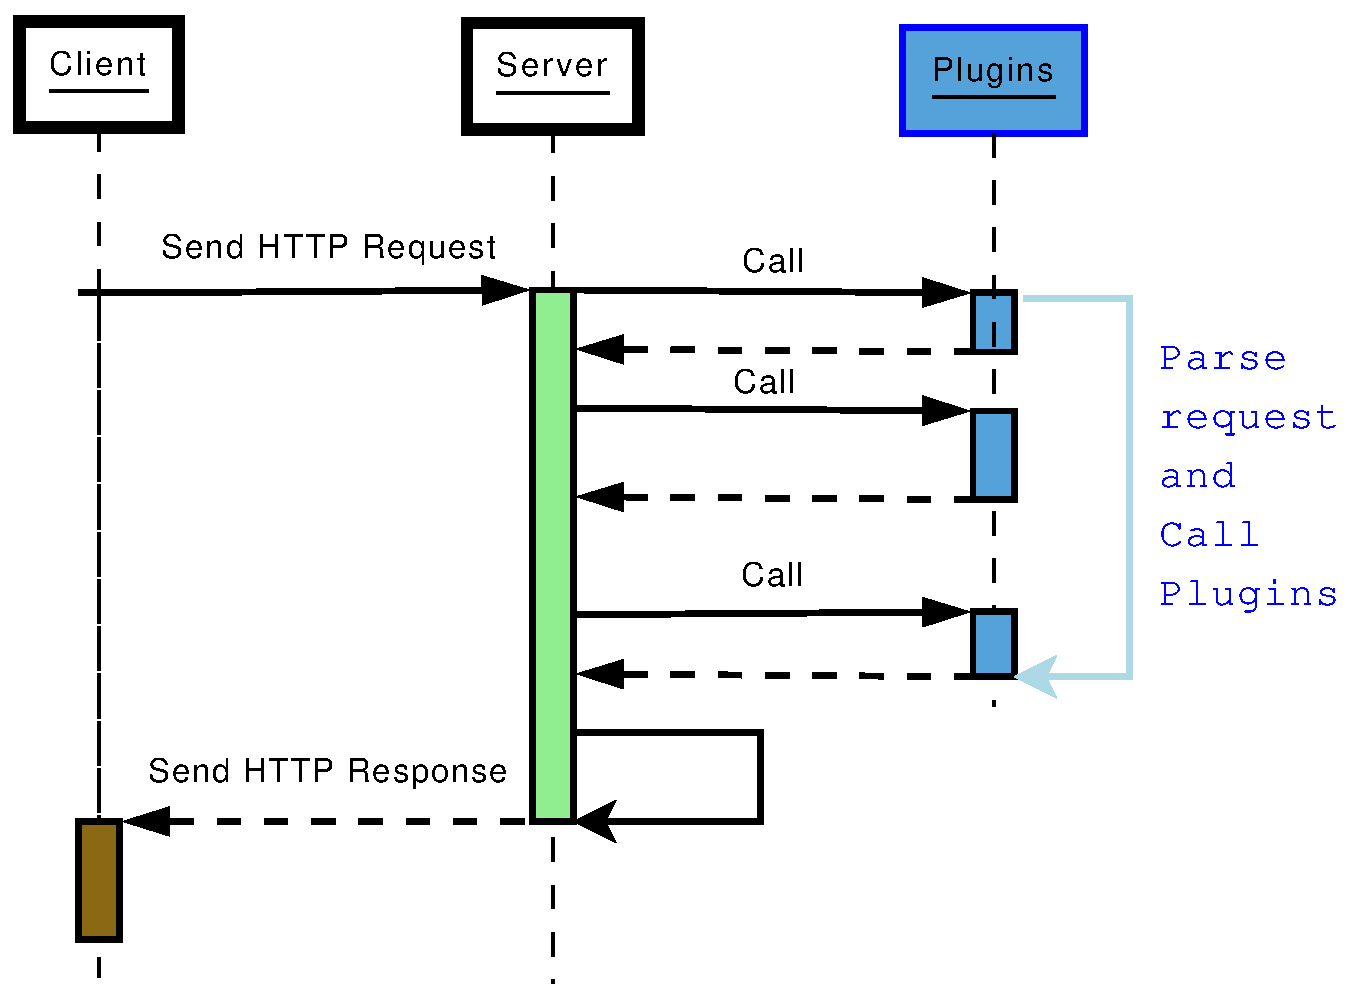
\includegraphics[height=9.5cm, width=12cm]{pics/httpplugin.eps}
	\end{figure}
	
	由于插件的具体功能对于服务器是透明的,服务器无法获知插件具体要对连接进行何种处理。服务器所知道的仅仅是插件所实现的接口。对于服务器而言,所有的插件都是一样的。当服务器处理某一个特定的请求时,服务器无法判断当前请求是否需要调用某一个插件进行处理。因此,服务器对于每一个请求,依次调用所有的插件。当某一个插件完成了对请求的处理之后,服务器将不在调用其他插件。服务器将这个插件的处理结果返回给客户端。那么,对于是否要对当前连接进行处理将有插件自己决定。比如,插件可以通过Request中的URI来判断是否需要对这个请求进行处理。
	
	由于插件的调用是按照一定的顺序进行的,因此,对于插件的调用就存在一个隐含的优先级。通常,最先加载的插件在处理请求的时候最先被调用。如果一个请求同时需要两个插件进行处理,那么,在第一个插件处理完毕之后,如果插件返回的是处理完毕,而不是继续处理,那么服务器将不会调用第二个插件进行处理。因此,通常情况下,插件处理完请求之后,应该告诉服务器继续调用其他插件处理请求,这样可以防止出现请求没有处理完毕的错误。
	
\subsection{插件接口的定义}
	插件接口被定义一些列标准函数原型。所有函数都有明确的定义和调用时机。这些函数大部分都是在前一节中描述的处理请求的过程中被调用。还有一些函数则在其他一些地方调用,以完成一些辅助的任务。下面详细介绍这些接口。
	
	首先,需要定义插件的初始化等函数。这些函数不用来处理请求,而是做一些辅助性的工作,不是在服务器处理请求的过程中被调用。
	\begin{itemize}
		\item init: 初始化插件。只调用一次,在加载插件之后调用。
		\item set\_default: 设置插件的配置为默认值。只调用一次,在加载插件之后调用。
		\item cleanup: 清理插件。在卸载插件的时候只调用一次。
		\item trigger: 每秒钟调用一次。相当于计时器。可以用来完成一些周期性的任务。
		\item sighup: 处理挂断信号。在服务器接收到这个连接的挂断信号(SIGHUP)时调用。
		\item connection\_close: 连接关闭时调用。
		\item connection\_reset: 连接重置时调用。
		\item joblist: 在连接被加入到作业队列中调用。作业队列中的连接处在等待I/O事件的状态。
	\end{itemize}
	
	下面需要定义在处理请求时所要调用的函数。在前面分析HTTP协议数据格式和处理过程可以看出,Request中的URI用来对所请求的资源进行定位。对于不同的资源,可以调用不同的插件进行处理。比如,如果请求的资源是以".o"为扩展名,那么就可以通过这一扩展名来判断所请求的是一个CGI脚本,还是一个普通文件。通常,以".o"为扩展名的是一个CGI脚本,那么就可以调用CGI插件进行处理。
	
	处理请求的函数如下:
	\begin{itemize}
		\item url\_raw: 获得原始的URI后调用。也就是未对“\% HEX HEX”形式的字符进行解码的URI。
		\item url\_clean: 获得已解码的URI后调用。
		\item docroot: 设置插件工作的根目录 。在获得解码后的URI后调用。
		\item physical: 获得请求资源对应的物理地址后调用。
		\item subrequest\_start: 子请求开始。
		\item handle\_subrequest: 处理子请求。
		\item subrequest\_end: 子请求结束。
	\end{itemize}
	
	最后三个处理子请求的函数在服务器处理请求的最后阶段分别调用。
	
	这些函数仅仅规定了其调用的时间,对于其具体的任务不做任何限定。比如,插件可以在调用physical接口函数的时候,查找所请求的资源,也可以在调用subrequest\_end时进行查找。同时,将接口细分之后,插件可以只对请求做部分的处理。例如,插件统计某一资源的请求次数时,可以在调用physical函数的时候完成,而不需要等到请求处理完毕。这样可以给予插件以较高的灵活性。
	
	对于每一个插件,这些接口函数都是选择性的进行实现。服务器会对插件所实现的接口函数进行记录。对于没有实现的接口函数,服务器将不会调用。
	
	由于插件接口有可能会因为需求的改变而随着服务器的不断升级而发生改变。对于一些使用旧版本的插件,很有可能在新版本的服务器中无法使用。因此,必须对插件的版本进行控制。
	
	插件的版本控制采用如下方法:插件版本号分为两个部分:主版本号和次版本号,两个版本号依次排列,并用'.'分割。比如:2.3,主版本号为2,次版本号为2。服务器的主次版本号和插件接口的主次版本号必须一致。主版本号改变通常由于插件接口发生了变化,不同主版本号的插件和服务器不兼容。次版本号改变通常是由于对插件的接口进行了增加,同时兼容较低次版本号的版本。次版本号底的插件同样可以运行在次版本号高的服务器上,当然,前提是主版本号相同。但是,不保证次版本号高的插件可以运行在次版本号底的服务器上。通常,服务器还有第三个版本号——BUG修正版本号,这个版本号不会对插件接口产生影响,仅仅是服务器的BUG修正。因此,不需要考虑到插件设计中。
	
\subsection{插件动态加载过程的分析和设计}
	为了进行动态的加载插件,服务器必须能实时的获知插件的增加。
	
	服务器可以通过检测插件的动态库所在的目录的变化,来获知是否有新的插件加入。但是,插件的动态库可能会放在不同的地方,这样就需要同时监测多个目录。这会影响服务器的效率。而且,一旦需要增加插件动态库存放的地方,必须通知服务器新增加的地方。这会增加服务器的复杂度。为了降低服务器的复杂度,本系统采用监测插件配置文件的方法。一旦插件配置发生更改(如,修改,删除等),服务器就重新读取插件配置文件,重新加载插件。监测的过程如图\ref{loadplugin}。
	\begin{figure}[htbp]
	\centering
	\caption{插件动态加载过程}
	\label{loadplugin}
	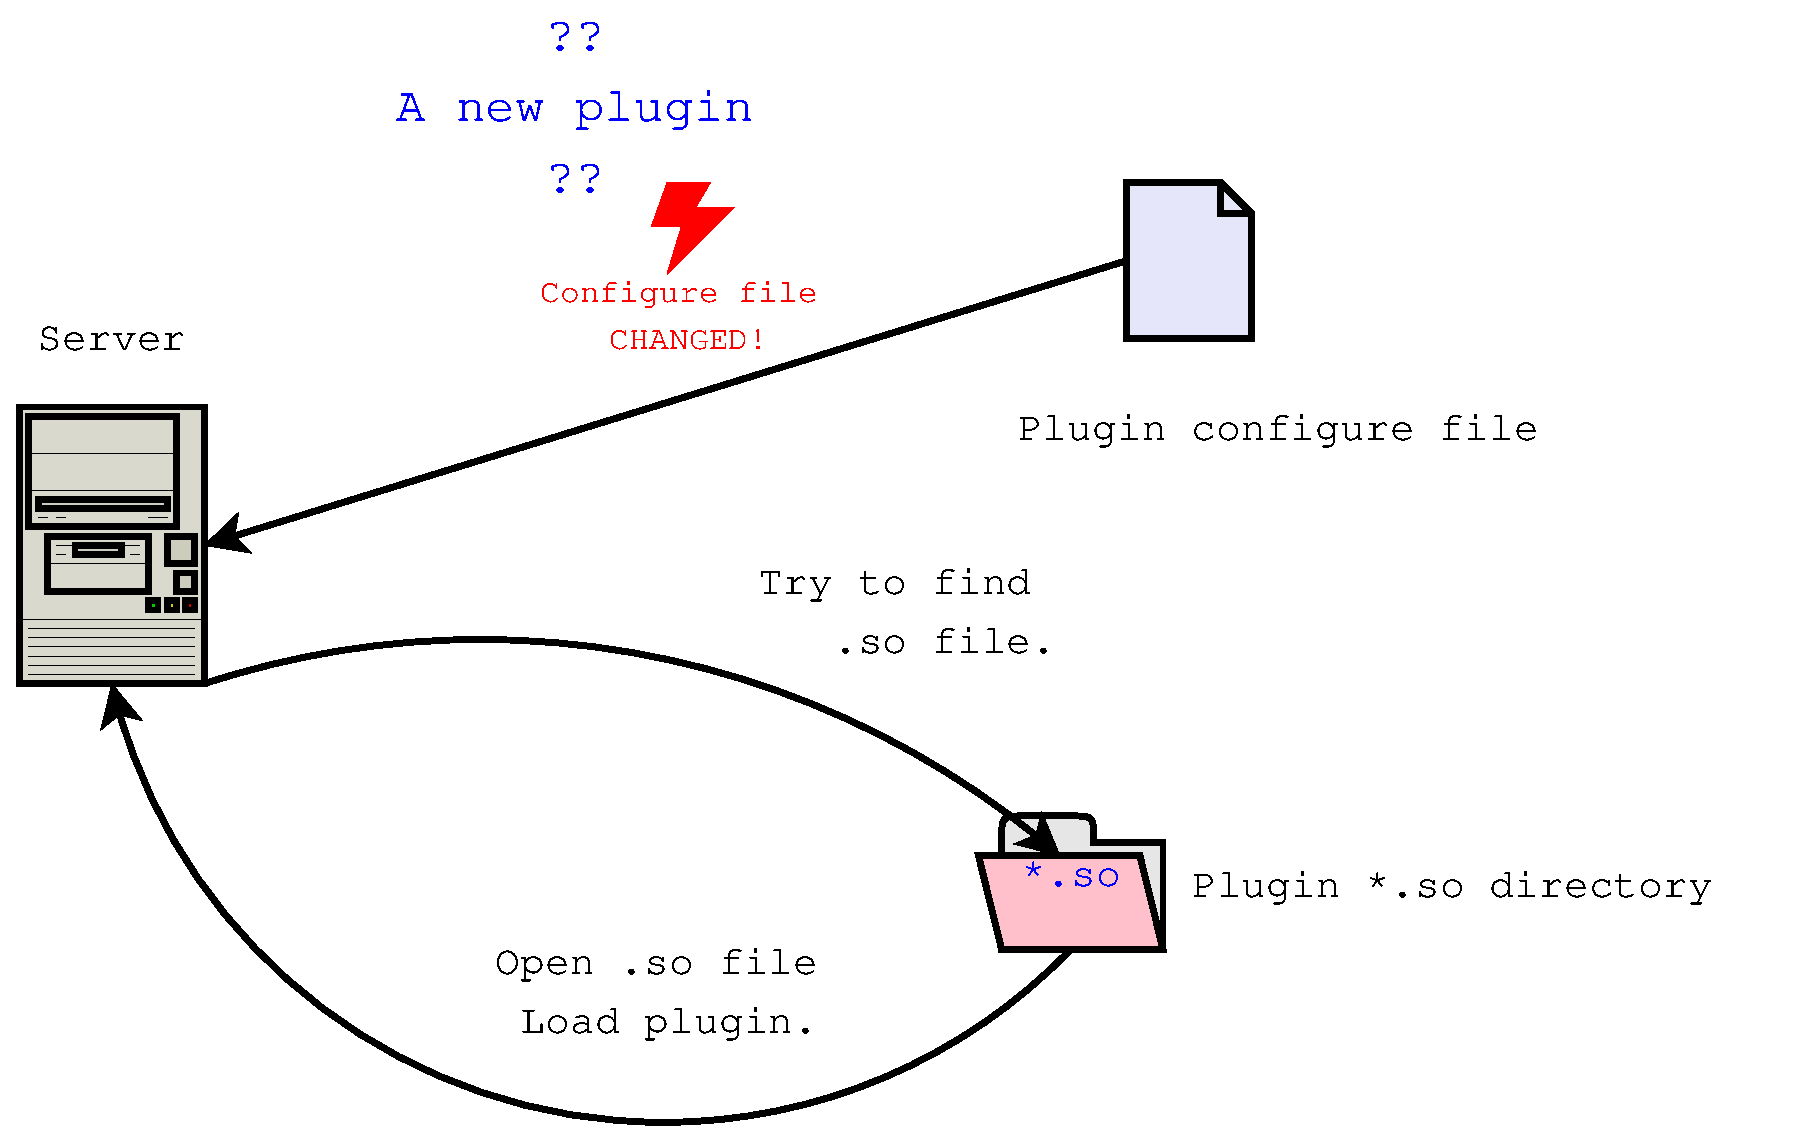
\includegraphics[height=8cm, width=13cm]{pics/loadplugin.eps}
	\end{figure}
	
	插件的加载和插件的调用是异步进行的。因此,在加载插件的时候,必须对插件的核心数据加锁,避免出现数据错乱导致服务器崩溃。
	
	动态链接技术可以选择性的加载共享库,也就是说,在程序的运行过程中,程序可以在任意时刻加载任意的共享库。动态链接技术的这个特点可以用来实现插件的加载。在服务器监测到插件的增加之后,通过配置文件中的信息,检索到插件的共享库,利用动态链接技术,将插件的共享库加载到内存中,并通知服务器插件接口的地址。服务器得到这些信息之后,就可以对插件进行调用。

\section{Web服务器的分析和设计}
\subsection{I/O分析和设计}
	Web服务器是I/O密集型的程序。在运行的大部分时间中,服务器都在进行这I/O处理。这些I/O处理包括接收和发送网络数据,读取和写入磁盘数据等。因此,服务器I/O效率的高低直接决定这服务器运行效率的高低。服务器在处理连接请求的时候,通常在某一时刻要同时处理多个请求,但这些请求并不是同时需要进行I/O。当某一个请求在等待I/O事件时,将这个请求暂时不处理,直到I/O事件发生再进行处理。在这个过程中,服务器对需要I/O的请求进行处理。这样可以增加服务器的吞吐量,提高效率。
	
	在本系统中,服务器的I/O处理采用非阻塞I/O+I/O多路复用+线程池的模式。对于所有的描述符,都将其设置为非阻塞模式,并通过I/O多路复用监测描述符的I/O事件。一旦某个描述符需要进行I/O,那么从线程池中获得一个线程,在这个线程中运行描述符对应的I/O处理函数。如果多个描述符同时需要I/O,可以实现并行处理,提高效率。I/O的结构图如图\ref{IO}。
	
	\begin{figure}[htbp]
	\centering
	\caption{I/O结构图}
	\label{IO}
	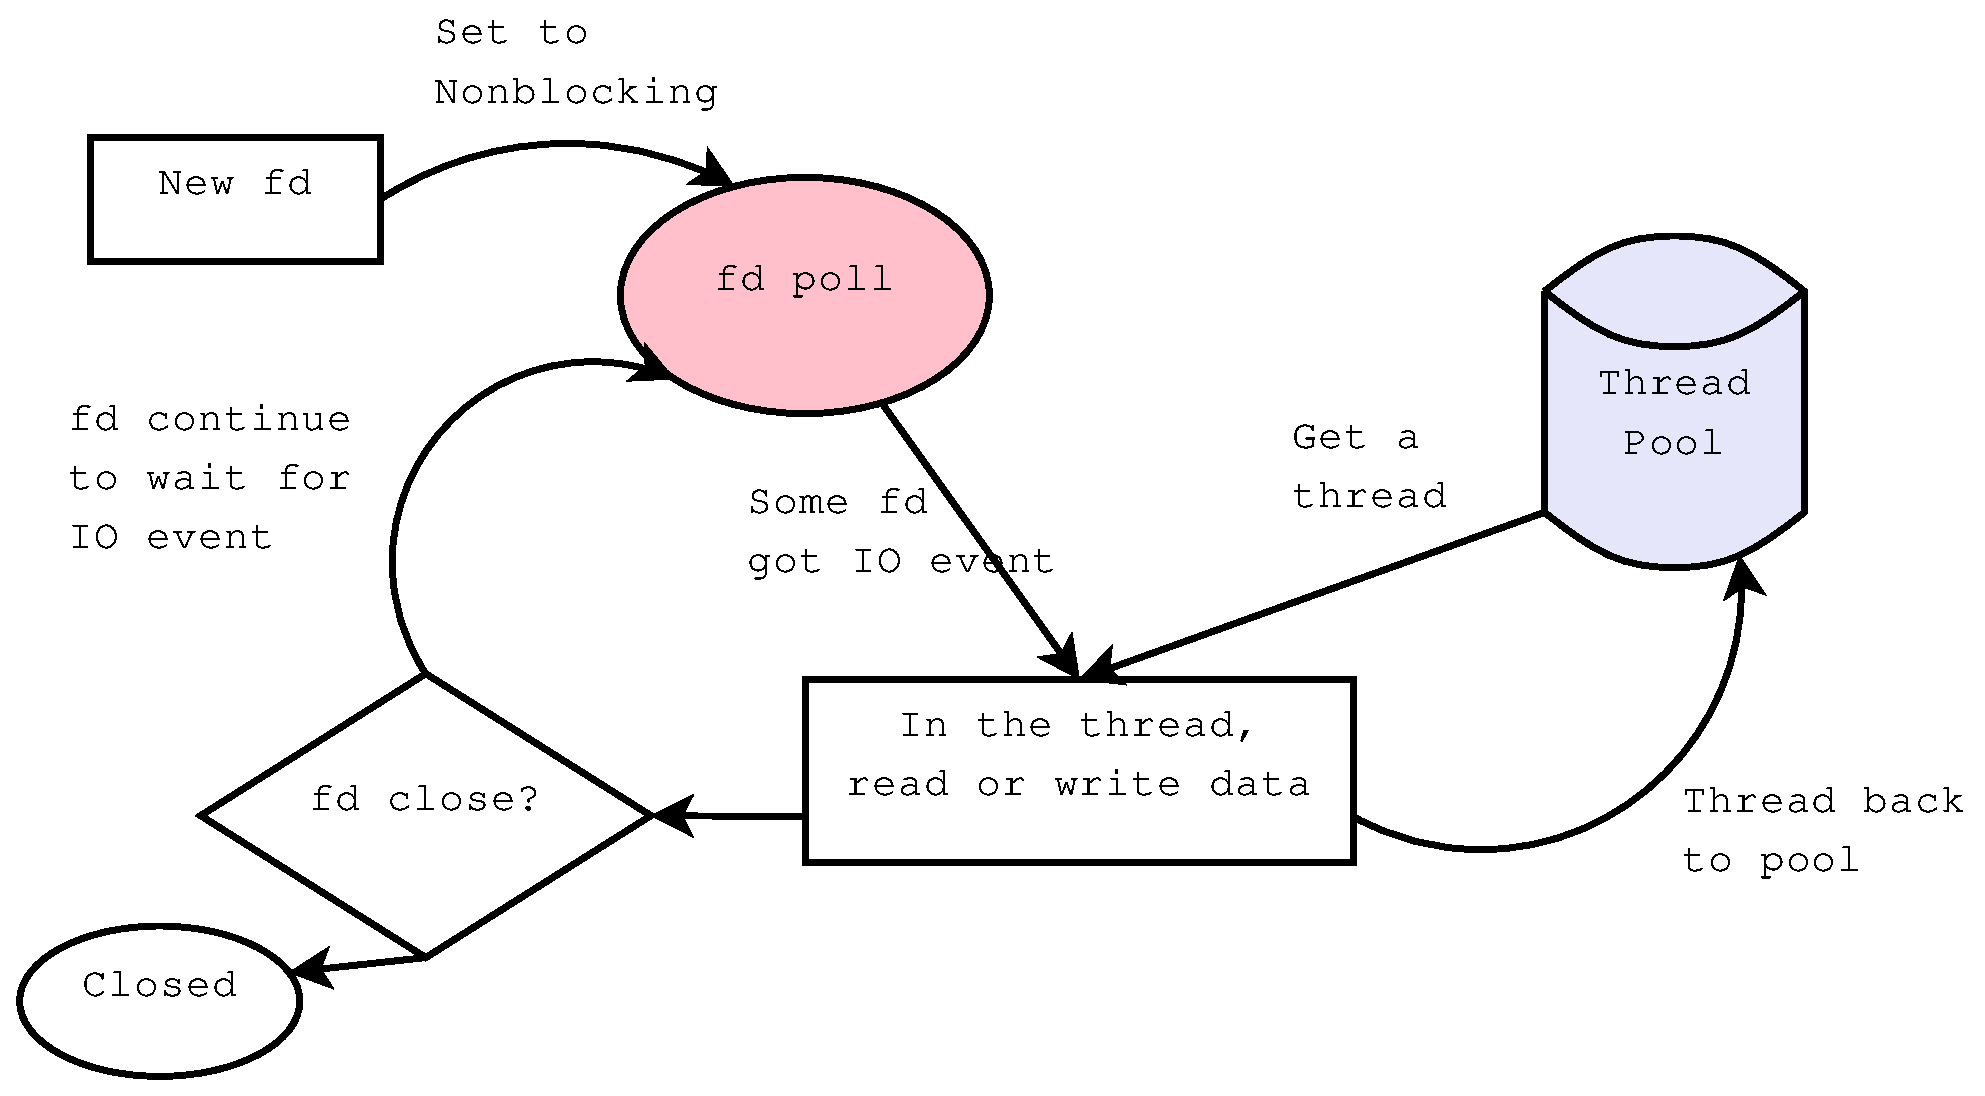
\includegraphics[height=8cm, width=15cm]{pics/IO.eps}
	\end{figure}
	
\subsection{线程池的设计}
	为了实现线程池的目的,必须能够控制线程使其在没有任务执行的时候处于等待状态(或者睡眠状态),而当有任务需要线程处理的时候,又可以快速的使线程恢复运行。当然,这里的运行只线程处于可运行状态(Running),是否真正运行要看线程调度程序对线程的调度。
	
	线程池具有如下特点:
	\begin{itemize}
		\item 在线程池的初始化阶段,预创建一些线程放入线程池中。
		\item 当线程池中没有可用线程时候,创建一个新的线程。这个新线程运行完任务之后,被加到线程池中,等待下一次调用。
		\item 当线程的总数量达到某一个最大值的时候,线程池将不在创建新的线程。如果此时没有可用线程,则请求线程的调用将阻塞,直到有线程可以使用。
		\item 当空闲线程较多时,将适当的销毁一些线程。通常,保证空闲线程的数量不会大于总的线程数量的2/3。
		\item 创建一个管理线程,对线程池进行管理。包括统计线程池的各种数据,销毁过多的空闲线程等。
	\end{itemize}
	
	在Linux下,使用Pthread库对线程进行创建管理等操作。Pthread库中的条件变量(Condition Variables)可以用来实现控制线程运行和等待的目的。条件变量可以使线程一直处于睡眠状态直到一些事件发生(或者条件改变)\ucite{unp}。线程处在一个循环中,循环的还是调用pthread\_cond\_wait等待有任务可以运行。此时,线程处于sleep状态。当有任务需要处理时,线程池调用pthread\_cond\_signal告诉线程有任务可以运行,唤醒线程。随后,线程处理任务。任务结结束后,线程再次回到sleep状态。线程的状态改变可用图\ref{tpthread}表示。
	
	\begin{figure}[htbp]
	\centering
	\caption{线程状态图}
	\label{tpthread}
	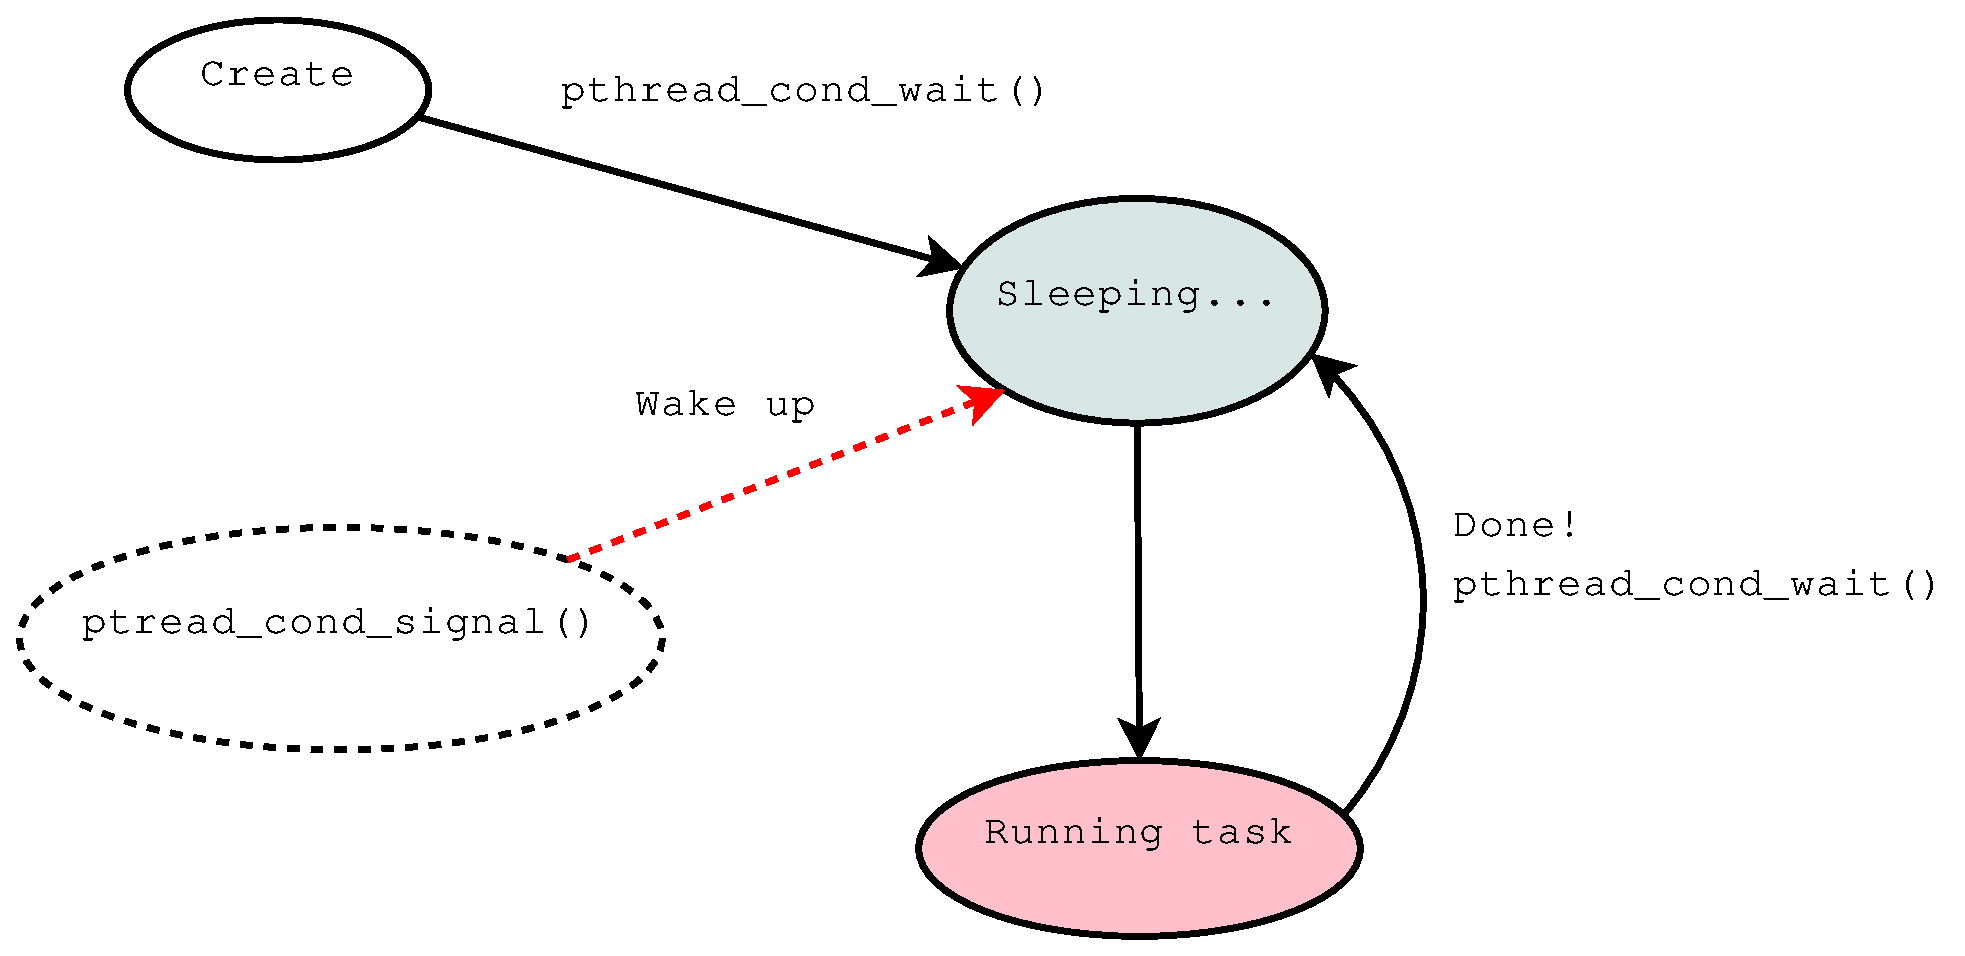
\includegraphics[height=6cm, width=13cm]{pics/tpthread.eps}
	\end{figure}
	
\subsection{连接处理状态机的设计}
	对于每一个请求,在不同的时刻,对请求所处在的状态进行定义。根据HTTP协议的规定,对于服务器而言,请求经历了读取Reqeust,解析Request,读取POST数据,处理连接请求,创建Response,发送Response回客户端这几个状态。为了便于处理,在请求的生命周期中增加了几个状态,最后的状态图如图\ref{state}。
	\begin{figure}[htbp]
	\centering
	\caption{请求处理状态图}
	\label{state}
	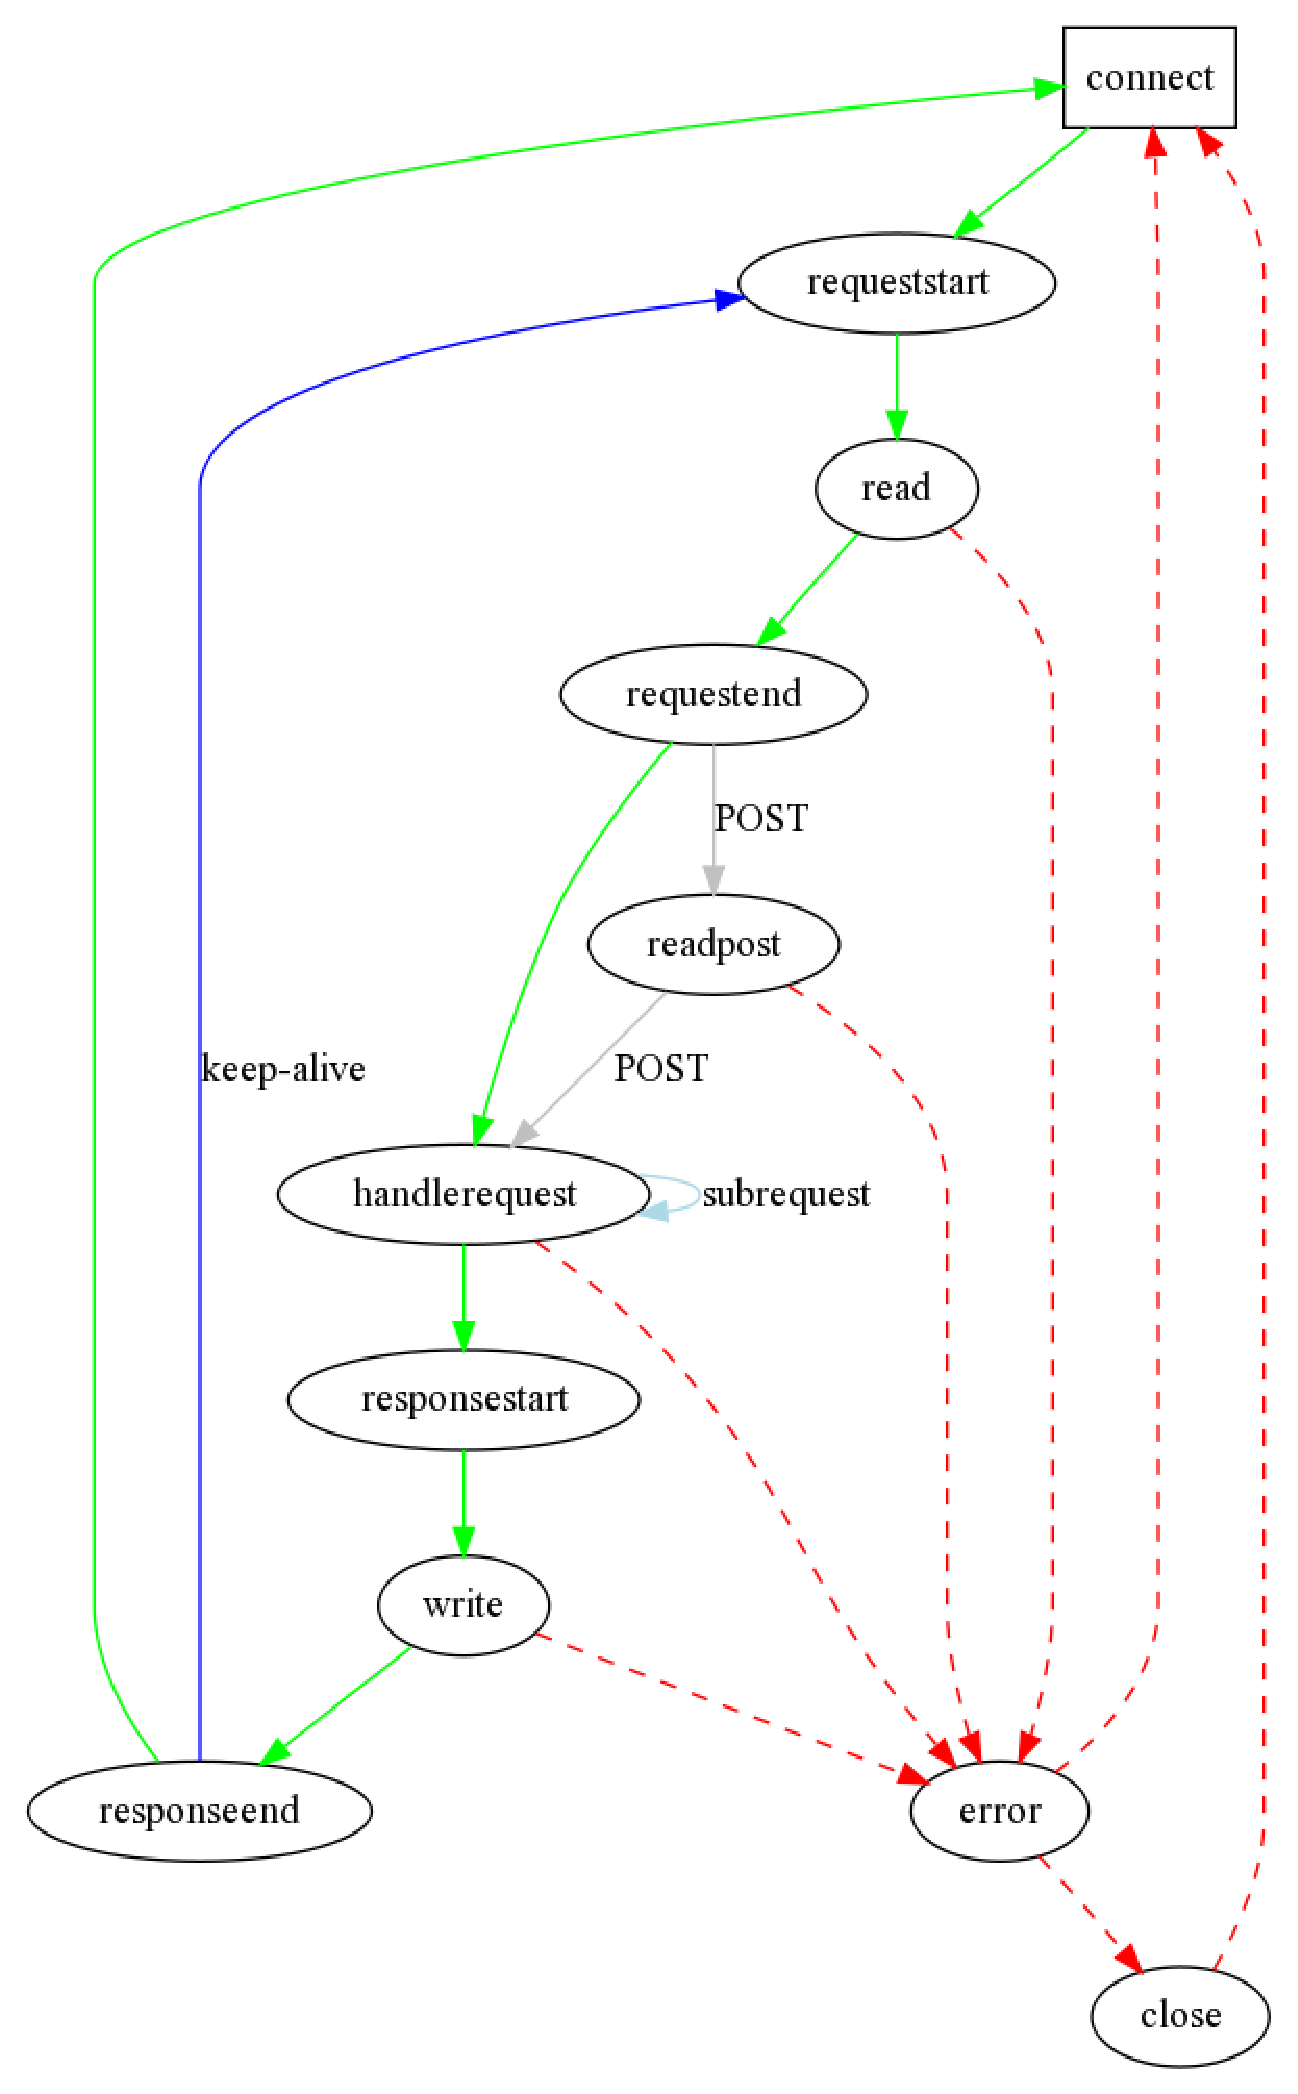
\includegraphics[height=22.5cm, width=14.5cm]{pics/state.eps}
	\end{figure}
	
	总共定义了10状态(图中椭圆所示)。connect状态是一个比较特殊的状态,它并不是请求在某一时刻的状态,它仅仅是用来标记连接对应的结构体可以使用。这个状态用来进行内部的数据处理,不参与请求的处理。
	
	各个状态的含义:
	\begin{itemize}
		\item connect: 标记connection结构体可用。
		\item requeststart: 请求开始。主要做一些时间的记录工作。
		\item read: 读取Request数据。
		\item handlerequest: 解析Request数据。
		\item requestend: 解析结束。做一些解析的收尾工作。
		\item readpost: 读取POST数据。如果没有POST数据,跳过此状态。
		\item responsestart: 处理请求。在这个状态中调用插件。这也是最重要的状态。
		\item write: 发送数据回client。
		\item responseend: 处理结束。做最后的清理工作。
		\item error: 出错。设置错误信息。
		\item close: 连接关闭。
	\end{itemize}
	
	图\ref{state}中虚线表示错误处理流程。一旦处理出错,服务器将关闭连接,不在接收这个连接的其余的请求。
	
	responseend状态结束后有两条路径:一条是标有keep-alve的指向requeststart状态的路径,一条是指向connect的路径。对于HTTP/1.1,通常是持久连接(Persistent Connection),也就是说,在处理完一个请求之后,连接不关闭。在此连接上可以再进行多次请求,直到连接双方有一方关闭了连接。如果连接不是持久连接,那么在处理完请求之后,服务器关闭连接。此时,请求已经处理完毕,不再需要任何状态表示。但是,为了方便内部数据的处理,将连接对应的结构体标记为connect状态。当有新的连接时,可以重新使用这个结构体。
	
	当请求处于handlerquest状态时,可能还需要进行子请求。这时候,请求依然处于handlerquest状态,并在这个状态中对子请求进行处理。某些请求可能会有多个子请求。这时,请求会一直停留在这个状态,处理所有子请求,然后进入下一个状态。
	
\chapter{插件接口和服务器的实现和测试}

\section{插件接口的实现}

\subsection{接口定义的实现}
	为了对插件进行描述,通过plugin结构体对插件进行封装。plugin结构体使用C语言的struct实现,包含有插件的所有信息。包括版本,名称,一系列接口函数指针以及一些辅助的数据成员。plugin结构体可以用图\ref{plugin_s}描述。
	
	\begin{figure}[htbp]
	\centering
	\caption{plugin结构体定义}
	\label{plugin_s}
	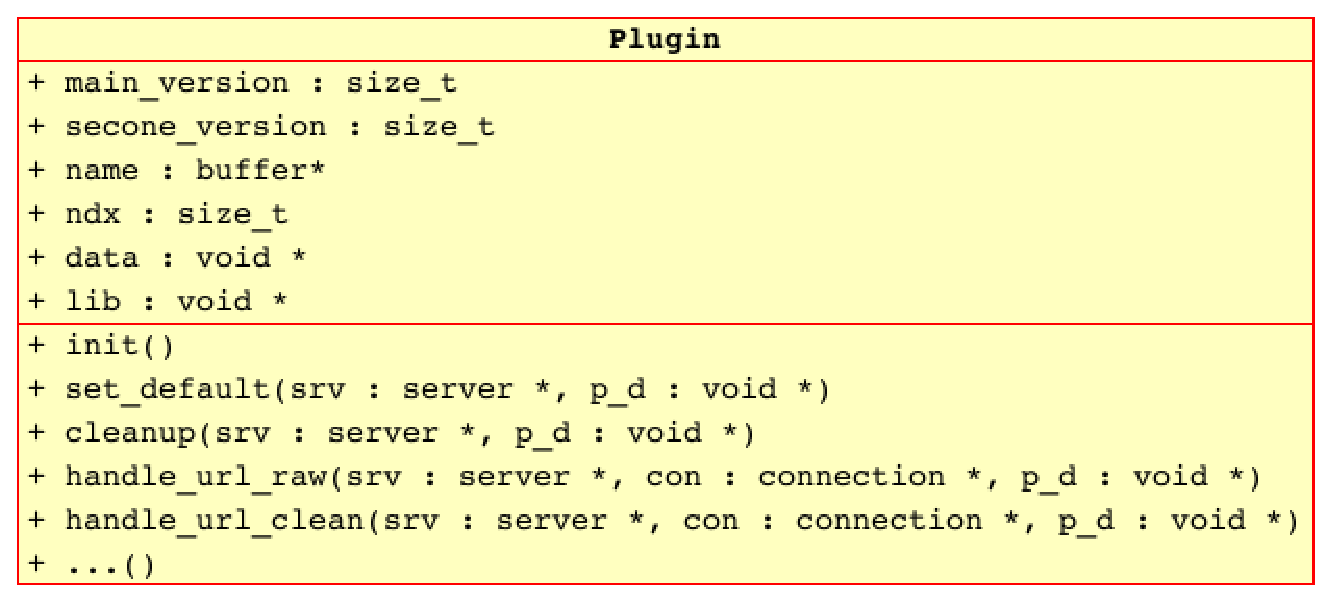
\includegraphics[height=6cm, width=12cm]{pics/plugin_s.eps}
	\end{figure}
	
	其中,main\_version和second\_version数据成员分别表示插件的主版本号和次版本号。服务器在加载插件的过程中,要对这两个版本号依据版本控制的规则进行检查。如果版本不兼容,则服务器不对插件进行加载,同时在日志文件中提示插件版本不兼容。
	
	name用来保存插件的名称。data指向插件自己使用的数据,和后面的函数指针中的p\_d参数对应。插件在初始化的过程中要自己分配所需要的数据空间,然后将地址赋给data。插件卸载时,要对这个数据空间进行释放。后面的一系列的函数指针保存着插件对应的函数的入口地址。每一个插件都要定义一个结构体plugin\_data用来存储插件所使用的私有数据。这个结构体的名称必须是plugin\_data,且在定义的开始部分一定是宏:PLUGIN\_DATA。插件在初始化的时候,要将这个结构体实例化并将其指针赋给plugin结构体中的data成员。宏PLUGIN\_DATA定义了一些数据成员。通过这一硬性规定,所有的插件的私有数据空间的开始部分都包含PLUGIN\_DATA所定义的数据成员。同时,插件系统自己也定义了一个plugin\_data结构体,这个结构体中只包含PLUGIN\_DATA定义的数据成员。插件系统通过把插件的数据空间强制转换成自己定义的plugin\_data结构体类型,就可以访问插件中这些有PLUGIN\_DATA定义的数据,从而实现对插件的一些管理。
	
	对于服务器而言,无论系统中有多少插件并且插件的接口实现个数都不相同,对于每个请求,服务器按部就班的调用所有插件接口函数。对于插件中的每一个接口函数,插件系统也定义了一些列的接口函数用于服务器调用插件。在调用插件时,服务器仅仅能看到这些接口,至于插件系统中到底有多少插件,服务器无法也不必知道。这些接口的定义如下:
	
\begin{verbatim}
handler_t plugin_handle_url_raw(server *srv, connection *con);
handler_t plugin_handle_url_clean(server *srv, connection *con);
handler_t plugin_handle_docroot(server *srv, connection *con);
handler_t plugin_handle_physical(server *srv, connection *con);
handler_t plugin_handle_connection_close(server *srv, connection *con);
handler_t plugin_handle_joblist(server *srv, connection *con);
handler_t plugin_handle_subrequest_start(server *srv, connection *con);
handler_t plugin_handle_handle_subrequest(server *srv, connection *con);
handler_t plugin_handle_request_end(server *srv, connection *con);
handler_t plugin_handle_connection_reset(server *srv, connection *con);

handler_t plugin_handle_trigger(server *srv);
handler_t plugin_handle_cleanup(server *srv);
\end{verbatim}
	在这些函数中,对每个插件的对应的接口函数进行调用。如果插件没有实现对应的接口函数,怎将忽略之。
	
\subsection{动态加载过程的实现}
	首先,定义插件的配置文件。插件的配置文件名字是固定的:swiftd-plugin.conf。插件配置文件存放的位置可以在服务器的配置文件中进行设置。配置文件的形式为”插件名称:插件动态库文件所在目录的绝对路径\$“。每一个插件,在配置文件中都有单独一行的这种形式的配置信息。例如:
	
	\begin{verbatim}
#以#开头的行为注释。swiftd-plugin.conf
#每个插件一行,每个插件配置信息必须以"$"结尾。
dir_index:/home/hcy/plugins/$
cgi:/home/temp/plugins/$
...
	\end{verbatim}

	这个例子中定义了两个插件:dir\_index和cgi。它们存放的位置分别是 /home/hcy/plugins/ 和 /home/temp/plugins/ 。
	
	插件的动态库的名称必须为:插件名称 +.so。服务器读取到插件配置信息之后,根据配置文件中的插件名称,可以确定插件的动态库的名称。这样就可以得到插件动态库的绝对路径。例如,上面两个插件的绝对路径分别为/home/hcy/plugins/dir\_index.so和/home/temp/plugins/cgi.so。
	
	服务器使用Linux平台下的Inotify技术对插件配置文件进行监测。Inotify产生一个文件描述符,通过监测这个文件描述符是否有数据可读即可监测到文件的改变。由于Inotify是根据文件描述符的有无数据可读来判断文件是否发生了改变。因此,可以将Inotify的描述符设置成非阻塞模式,然后利用服务器中的I/O多路复用来监测其描述符的I/O事件 。这样,可以实现对配置文件修改的异步实时监测,同时,也不会影响服务器的效率。监测过程如图\ref{inotify}。
	
	\begin{figure}[htbp]
	\centering
	\caption{Inotify监测过程}
	\label{inotify}
	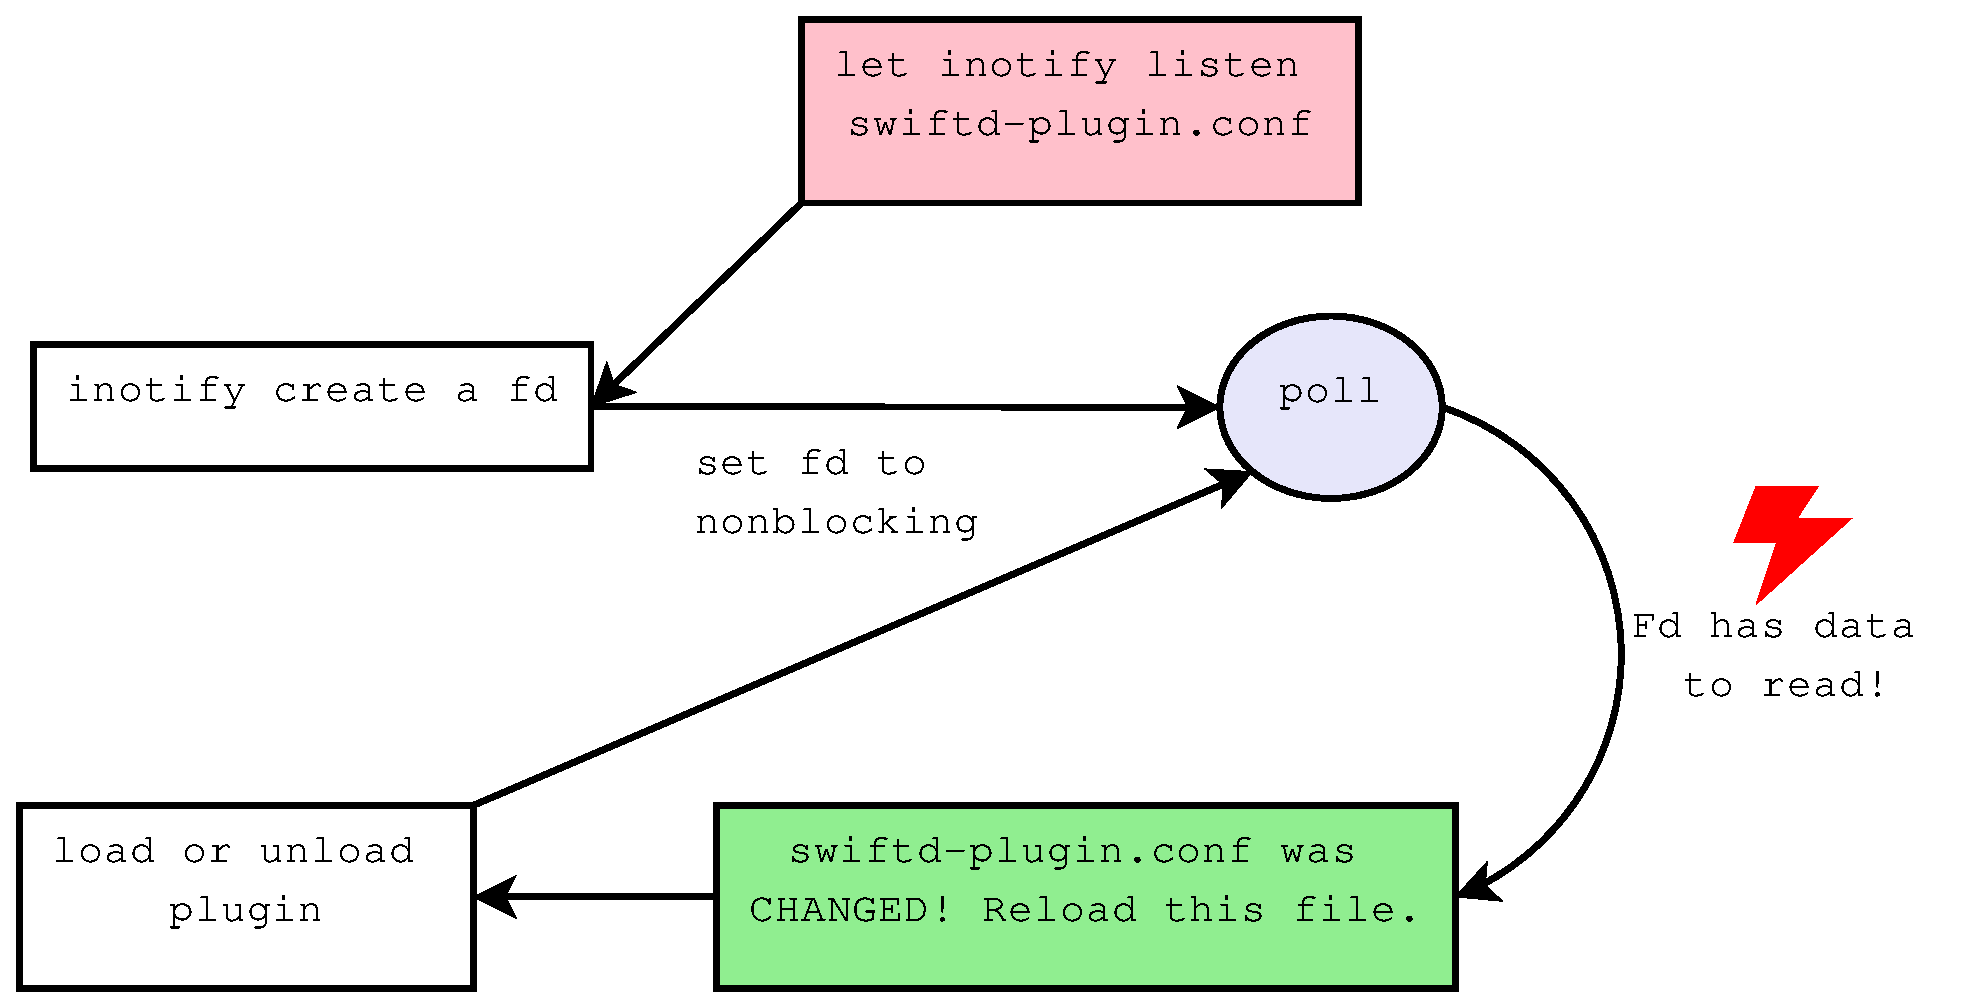
\includegraphics[height=8cm, width=15cm]{pics/inotify.eps}
	\end{figure}
	
	\begin{enumerate}
		\item 在服务器初始化阶段,调用inotify\_init()创建一个Inotify实例。此时函数返回一个文件描述符fd。
		\item 调用inotify\_add\_watch()对插件配置文件所在的目录监测IN\_CLOSE\_WRITE事件(参见后文)。
		\item 将inotify\_init()返回的文件描述符fd和对应的I/O事件处理函数\\plugin\_conf\_inotify\_fdevent\_handler()注册到I/O多路复用系统中。由I/O多路复用监测fd的I/O事件。
		\item 配置文件被修改。调用fd的I/O事件处理函数。在这个处理函数中重新加载所有插件。
		\item fd重新进入等待I/O事件状态。
	\end{enumerate}
	
	对于有些编辑器(如,vi),在对文件进行编辑的时候并不是在原文件上进行修改,而是首先复制一个文件的副本,然后在这个副本上进行编辑操作。当编辑完毕之后,用这个副本覆盖原来的文件。如果直接监测对应文件的IN\_MODIFY事件,那么,在进行文件覆盖时,监测到文件被删除,Inotify将停止对文件的监测,也就是相当于inotify\_rm\_watch文件了。这样,就只能监测到一次IN\_DELETE\_SELF事件。随后什么也监测不到。为了能够对文件进行正常的监测,这里不直接监测文件,而监测包含文件的文件夹。一旦文件被覆盖,将触发文件夹IN\_CLOSE\_WIRTE事件。这样即可得到文件的修改事件。
	
	为了能对插件进行初始化并得到其所实现的接口函数的入口地址。规定所有的插件中必须实现一个函数XXXXXX\_init,其中,	XXXXXX为插件的名称(必须为插件配置文件中的名称)。这个函数的原型为:
	\begin{verbatim}
        void XXXXXX_init(plugin *p)
	\end{verbatim}
	
	在这个函数中,主要而且必须的工作就是对所传进来的plugin结构体的数据成员进行赋值。其中,最重要的是版本和接口函数指针的赋值。如果插件没有实现某一个接口函数,那么那么接口函数对应的函数指针必须赋值为NULL。这点很重要。在插件系统得到了插件动态库的路径之后,通过dlopen调用将动态库加载到内存中。然后,插件系统通过dlsym调用获得插件对应的XXXXXX\_init函数的入口地址。接着插件系统创建一个plugin结构体的实例,并以这个实例的地址为参数调用刚才得到的XXXXXX\_init函数。至此,插件系统得到了插件的所有信息。完成了插件的加载工作。
	
\subsection{插件调用的实现}

	首先,为了对插件的各个接口进行标记,程序中定义了一个枚举类型plugin\_slot\_t。定义如下:
\begin{verbatim}
typedef enum
{
	PLUGIN_SLOT_SET_DEFAULT= 0,
	PLUGIN_SLOT_CLEANUP,
	PLUGIN_SLOT_TRIGGER,
	PLUGIN_SLOT_SIGHUP,
	PLUGIN_SLOT_URL_RAW,
	PLUGIN_SLOT_URL_CLEAN,
	PLUGIN_SLOT_DOCROOT,
	PLUGIN_SLOT_PHYSICAL,
	PLUGIN_SLOT_JOBLIST,
	PLUGIN_SLOT_CONNECTION_CLOSE,
	PLUGIN_SLOT_CONNECTION_RESET,
	PLUGIN_SLOT_SUBREQUEST_START,
	PLUGIN_SLOT_HANDLE_SUBREQUEST,
	PLUGIN_SLOT_SUBREQUEST_END,
	PLUGIN_SLOT_SIZE, 			//slot的数量。
}plugin_slot_t;
\end{verbatim}

	这个枚举类型中的值与接口函数有这对应关系。从这些值的名称中可以得知。比如,PLUGIN\_SLOT\_DOCROOT对应于docroot接口函数。
	
	然后,为了提高插件的调用效率,对每一个插件进行登记造册。plugin\_slot是一个void *类型的二维数组,相当于plugin的登记表。当插件加载之后,插件所有的信息都存放在对应的plugin结构体中。插件系统遍历所有的plugin结构体,对插件所实现的接口方法进行登记(前面已经说过,对于没有实现的插件接口,插件必须将对应的函数指针赋值为NULL。这就可以帮助插件系统判断插件到底实现了哪些接口函数)。
	
	plugin\_slot虽说是一个void*类型的数组,但是其存放的是plugin结构体的插件。plugin\_slot数组的每一行对应一个接口函数。对应关系由plugin\_slot\_t枚举类型确定。比如,根据C语言语法规定,枚举值PLUGIN\_SLOT\_DOCROOT等于6。那么docroot接口函数对应的行就是第7行(C语言从第0行开始计算),换句话说,第7行中保存这所有实现了docroot接口函数的插件的plugin结构体指针。
	
	例如,目前有三个插件,它们登记之后plugin\_slot数组的情况可有表\ref{example_plugin}表示。
	\begin{table}[htbp]
	\caption{plugin\_slot示例:}
	\label{example_plugin}
	\centering
	\begin{tabularx}{\textwidth}{p{6cm}XXXl} %最后一列是空的。这样可以是倒数第二列居中,否则会报错或不居中。
	\toprule
	\centering 名称 & \centering  插件1 & \centering  插件2 &\centering 插件3&\\
	\midrule
	\centering PLUGIN\_SLOT\_PHYSICAL &\centering  p1 &\centering  p2 &\centering  p3&\\
	\centering PLUGIN\_SLOT\_URI\_CLEAN &\centering  p1 &\centering  p2 &\centering  p3&\\
	\centering PLUGIN\_SLOT\_DOCROOT &\centering  p1 & \centering NULL & \centering NULL&\\
	\bottomrule
	\end{tabularx}
	\end{table}
	
	NULL表示插件没有实现对应的接口函数。px表示插件对应的plugin结构体指针。
	
	表\ref{example_plugin}中仅仅示例了三个接口函数。从表\ref{example_plugin}可以看出,插件1实现了全部的三个接口函数,插件2没有实现第三个接口函数,插件3和插件2一样。插件系统利用如下的宏对插件进行登记:
	
\begin{verbatim}
#define PLUGIN_REGISTER_SLOT(x, y)\
 for(i = 0; i < srv -> plugins -> used; ++i)\
 {\
  plugin *p = srv -> plugins -> ptr[i];\
  if(p -> handle_##y)\
  {\
   log_error_write(srv, __FILE__, __LINE__, \
   			"sb", "slot: ", p -> name);\
   if(NULL == srv -> slots -> size)\
   {\
    srv -> slots -> used = (size_t *)\
    			calloc(PLUGIN_SLOT_SIZE, sizeof(size_t *));\
    srv -> slots -> size = (size_t *)\
    			calloc(PLUGIN_SLOT_SIZE, sizeof(size_t *));\
	srv -> slots -> ptr = (void ***)\
				calloc(PLUGIN_SLOT_SIZE, sizeof(void **));\
   }\
   if (srv -> slots -> size[x] == 0)\
   {\
	srv -> slots -> size[x] = 8;\
	srv -> slots -> ptr[x] = (void **)\
			calloc(srv -> slots -> size[x], sizeof(void *));\
   }\
   else if (srv -> slots -> size[x] == srv -> slots -> used[x])\
   {\
	srv -> slots -> size[x] += 8;\
	srv -> slots -> ptr[x] = (void **)realloc(\
			srv -> slots -> ptr[x],\
			srv -> slots -> size[x] * sizeof(void *));\
   }\
   srv -> slots -> ptr[x][srv -> slots -> used[x]] = (void*)p;\
   ++srv -> slots -> used[x];\
  }\
 }
\end{verbatim}
	
	宏的第一个参数x确定需要登记的接口函数的类型,这个参数是plugin\_slot\_t类型。第二个参数y是x对应的接口函数在pluing结构体中对应的数据成员的名称不包含开头的handle\_。宏中扫描所有的插件,如果插件实现了x对应的接口函数,就将这个插件对应的plugin结构体指针存入plugin\_slot数组中。宏中还包含了对plugin\_slot数组空间申请。
	
	例如,这个宏调用实现对docroot接口函数的登记工作。
	\begin{verbatim}
	PLUGIN_REGISTER_SLOT(PLUGIN_SLOT_DOCROOT, handle_docroot);
	\end{verbatim}
	
	得到这张登记表之后,基本上所有的操作都是围绕这个表来进行的。插件系统定义了下面的宏,这个宏用来作为模板,实现先前提到的插件系统提供给服务器的那一些列接口函数。而这些接口函数是服务器调用插件的关键。

\begin{verbatim}
#define PLUGIN_CALL_HANDLER(x,y)\
 handler_t plugin_handle_##y(server *srv, connection *con)\
 {\
  if (NULL == srv || NULL == con)\
  {\
   return HANDLER_ERROR;\
  }\
   \
  if (!srv -> slots -> ptr)\
  {\
   return HANDLER_GO_ON;\
  }\
  if (!srv -> slots -> ptr[x])\
  {\
   return HANDLER_GO_ON;\
  }\
   \
   pthread_mutex_lock(&srv -> plugin_lock);\
   plugin *p;\
   size_t i;\
   handler_t ht;\
   for (i = 0; i < srv -> slots -> used[x]; ++i)\
   {\
	if (srv -> slots -> ptr[x][i])\
	{\
	 p = (plugin*)srv -> slots -> ptr[x][i];\
	 switch(ht = p -> handle_##y(srv, con, p -> data))\
	 {\
	  case HANDLER_GO_ON:\
	    break;\
	  case HANDLER_FINISHED:\
	  case HANDLER_COMEBACK:\
	  case HANDLER_WAIT_FOR_EVENT:\
	  case HANDLER_ERROR:\
	  case HANDLER_WAIT_FOR_FD:\
		pthread_mutex_unlock(&srv -> plugin_lock);\
		return ht;\
	  default:\
		log_error_write(srv, __FILE__, __LINE__, \
						"Unknown handler type.");\
		pthread_mutex_unlock(&srv -> plugin_lock);\
		return HANDLER_ERROR;\
	  }\
     }\
   }\
   pthread_mutex_unlock(&srv -> plugin_lock);\
   return ht;\
 }
\end{verbatim}	
	
	宏的第一个参数x确定需要登记的接口函数的类型,这个参数是plugin\_slot\_t类型。第二个参数y是x对应的接口函数在pluing结构体中对应的数据成员的名称不包含开头的handle\_。在这个宏中,通过x确定pluing\_slot数组的行,依次调用这行中存储的plugin结构体的对应的成员函数(函数指针)。这些成员函数的名称有y确定。这一调用工作,正是插件系统提供给服务器的所有接口函数的全部工作。利用这个宏,可以模板化的实现所有这些函数。例如,宏调用
	
	\begin{verbatim}
	PLUGIN_CALL_HANDLER(PLUGIN_SLOT_DOCROOT, docroot);
	\end{verbatim}
	
	将这个宏展开就得到了plugin\_handle\_docroot函数的完整定义。
	
	当请求进入reponsestart状态(图\ref{state})时,服务器调用http\_prepare\_response函数。在这个函数中,解析Resquest中的URI。在解析的过程中,按照插件接口的定义,在完成某一解析步骤之后,调用插件接口函数,调用插件处理请求。
	
\section{服务器的实现}

\subsection{I/O实现}
	首先,对I/O多路复用进行包装。这样可以实现使用不同的I/O多路复用实现时,对服务器而言有一个统一的接口。用户可以在对服务器编译阶段,通过定义不同的宏来选择系统中包含哪些实现。默认情况下使用的是Linux下的epoll。下面这个结构体描述了服务器的I/O多路复用系统:
	
\begin{verbatim}	
typedef struct fdevent
{
	fdevent_handler_t type;
	fdnode *fdarray;
	size_t maxfds;
	pthread_mutex_t lock; //锁

#ifdef USE_EPOLL
	int epoll_fd;
	struct epoll_event *epoll_events;
#endif
#ifdef USE_SELECT
	//用于传递给select函数。
	fd_set select_read;
	fd_set select_write;
	fd_set select_error;
	//select函数会改变上面三个函数,在这保留一个副本。
	fd_set select_set_read;
	fd_set select_set_write;
	fd_set select_set_error;
	//select函数的第一个参数。
	int select_max_fd;
#endif
	int (*reset)(struct fdevent *ev);
	void (*free)(struct fdevent *ev);
	int (*event_add)(struct fdevent *ev, int fd, int events);
	int (*event_del)(struct fdevent *ev, int fd);
	int (*event_get_revent)(struct fdevent *ev, int ndx);
	int (*event_get_fd)(struct fdevent *ev, int ndx);
	int (*event_get_next_ndx)(struct fdevent *ev, int ndx);
	int (*poll)(struct fdevent *ev, int timeout);
	int (*fcntl)(struct fdevent *ev, int fd);
}fdevent;
\end{verbatim}

	结构体中的宏可以在服务器使用不同I/O多路复用实现时,结构体包含不同的数据成员。如果系统中有多个实现,那么结构体中也可以包括多个实现所需要的数据。最终使用哪个实现,由type决定。这个可以在配置文件中进行设置。type的值决定了初始化函数中对哪个I/O多路复用实现进行初始化。type是一个枚举类型变量。
	
	结构体最后的一系列函数指针类似于成员函数。当是使用不同的I/O多路复用实现时,函数指针中存放的是对应的各个函数的入口地址。对于不同的I/O多路复用实现,都有与这几个函数指针对应的函数定义。在初始化的时候,服务器根据所使用的I/O多路复用实现,对这些函数指针赋予不同的值。在服务器运行阶段,服务器不需要知道所使用的I/O多路复用的具体情况,仅仅通过这几个函数指针调用对应的函数来完成I/O监听任务。为了方便服务器的调用,在实现中对这几个函数指针进行了一次包装。也就是,定义了一系列接口函数,在这些函数中调用这些函数指针。而服务器只需要调用这些接口函数。接口函数的声明如下:
	
\begin{verbatim}
int fdevent_reset(fdevent *ev);
void fdevent_free(fdevent *ev);
int fdevent_event_add(fdevent *ev, int fd, int events);
int fdevent_event_del(fdevent *ev, int fd);
int fdevent_event_get_revent(fdevent *ev, int ndx);
int fdevent_event_get_fd(fdevent *ev, int ndx);
int fdevent_event_get_next_ndx(fdevent *ev, int ndx);
int fdevent_poll(fdevent *ev, int timeout);
int fdevent_fcntl(fdevent *ev, int fd);
\end{verbatim}

	在程序的主循环中,接口函数的调用过程如下:

\begin{verbatim}
	do
	{
		n = fdevent_poll(srv -> ev, 1000);
		ndx = -1;
		while(--n >= 0)
		{
			ndx = fdevent_event_get_next_ndx(srv -> ev, ndx);
			fd  = fdevent_event_get_fd(srv -> ev, ndx);
			revents = fdevent_event_get_revent(srv -> ev, ndx);
			handler = fdevent_event_get_handler(srv -> ev, fd);
			ctx = fdevent_event_get_context(srv -> ev, fd);			
			
			//调用线程处理I/O事件。
		}
	}while(!shutdown_server);
\end{verbatim}	
	
	fdevent\_poll函数用来开始监听所有注册的描述符。通常,程序阻塞在这个函数中,直到有描述符发生了I/O事件或者等待超时。当有描述符发生I/O事件时,通过接口函数,获得发生I/O事件的描述符和所发生的事件,以及其对应的事件处理函数。最后,调用线程处理I/O事件。fdevent\_poll函数被设定为等待1s后超时。如果1s后没有I/O事件发生,那么fdevent\_poll函数将返回。通过这个超时设置,可以实现一个粗略的计时器。通过这个计时器,可以做一些秒一级的计时工作。
	
	在这些接口函数中,大部分的任务仅仅是调用了这些函数指针对应的函数。增加这一层包装,进一步隐藏I/O多路复用系统的实现细节,降低程序的耦合性。

	对于每一种描述符,服务器中都定义了一个与之对应的I/O事件处理函数。当描述符发生了I/O事件时,服务器通过调用与这个描述符对应的处理函数处理I/O事件。对于这个处理函数,定义了如下的原型:
	
\begin{verbatim}	
typedef handler_t (*fdevent_handler)(void *srv, void *ctx, int revents);
\end{verbatim}
	
	通过定义这样一个函数原型,强制所有的I/O处理函数都必须有一致的形式。这样,当服务器调用处理函数处理I/O事件时,不需要区分到底是哪种描述符发生了I/O事件。服务器与I/O多路复用系统的耦合度进一步的降低。
	
	最后,对于每一种I/O多路复用实现,对于I/O事件的定义都不尽相同。因此,为了对这些实现差异进行隐藏,服务器中定义了自己的一套I/O事件定义。对于不同的I/O多路复用实现,要将其I/O事件的定义与之对应。而这些对应关系和装换,则完全隐藏在具体的实现中。服务器只需要关系接口函数返回的事件。
	
	在服务器的实现中,使用一个整数类型的不同的位表示不同的事件。具体的定义如下:
\begin{verbatim}	
#define BV(x) (1 << x)

#define FDEVENT_IN	  BV(1) 	//fd可写
#define FDEVENT_OUT 	BV(2) 	//有数据可读
#define FDEVENT_ERR 	BV(3) 	//出错
#define FDEVENT_PRI 	BV(4) 	//有不阻塞的可读的高优先级数据。
#define FDEVENT_HUP 	BV(5) 	//已挂断
#define FDEVENT_NVAL	BV(6) 	//描述符不引用一个打开文件。
\end{verbatim}
	
	这样定义事件,即节省内存,又可以通过或运算在一个整数类型变量中表示多个事件。当一个描述符同时发生了多个事件时,这种定义可以方便的在一个变量中表示这多个事件。对于函数的定义有很大的帮助。当然,如果I/O事件较多,可能一个整型变量表示不了这么多,那么就必须使用其他方法来解决。在本系统中,值定义了6中I/O事件,在32位系统上用整型变量表示不存在这个问题。
	
\subsection{线程池的实现}
	为了便于管理和隐藏实现细节,同样,使用一个结构体表示线程池:
\begin{verbatim}
\begin{verbatim}
struct s_thread_pool
{
	pthread_mutex_t lock; 
	int max_num;            //最大线程数。
	int min_num;            //最小线程数。
	int cur_num; 
	thread_info *threads;
	sem_t thread_cnt_sem;   //用于达到线程最大值且还有作业时,等待线程空闲。
};
\end{verbatim}
	
	这个结构体中最重要的数据成员是threads数组。这个数组中存放着线程池中所有线程的信息。其定义如下:

\begin{verbatim}	
typedef struct 
{
	pthread_t id; 
	int ndx;              //在数组threads中的位置。
	pthread_mutex_t lock; 
	pthread_cond_t  cond; //条件变量。用于等待作业分配。
	thread_pool *tp;
	int stop;
	int is_busy;
	job_func job;         //线程需要执行的作业
	void *ctx;            //执行作业需要的数据.
}thread_info;
\end{verbatim}

	这个结构体中保存了线程的一些重要的信息,包括线程id,在threads数组中的下标等。job成员变量是一个函数指针,这个指针的原型为:
\begin{verbatim}
	typedef void *(*job_func)(void *ctx); 
\end{verbatim}

	在每个线程中,当有任务去需要执行的时候,线程回去执行这个指针所指向的函数。通过定义这个指针,可以强制所有需要线程处理的任务都具有相同的形式。当线程处理任务的时候,不需要知道具体是什么任务。参数ctx通常指向一个结构体,这个结构体中保存着任务所需要的一些信息。这个结构体的指针保存在thread\_info结构体的ctx变量中。当线程执行任务时,把这个变量作为参数传递给job所指向的函数。
	
	线程池的接口函数很简单,只有三个:
\begin{verbatim}
thread_pool* tp_init(int minnum, int maxnum);
void tp_free(thread_pool *tp);

int tp_run_job(thread_pool *tp, job_func job, void *ctx);
\end{verbatim}

	前面两个是初始化和释放函数,初始化函数的参数表示线程池中线程的最小值和最大值。在服务器的运行过程中只执行一次。第三个函数是在线程池中获得一个线程,然后执行参数job指向的函数(任务),参数ctx是这个函数的运行参数。tp\_run\_job函数首先查找空闲的线程,如果没有空闲线程则创建一个。如果线程书达到最大数量且没有空闲线程,那么函数阻塞,直到有线程空闲可用。当找到一个线程之后,tp\_run\_job函数将其后两个参数分别赋值给线程对应的结构体的job成员和ctx成员,最后,通过pthread\_cond\_signal函数通知线程执行任务函数。
	
	当线程启动之后,线程就一直运行在下面的循环中:

\begin{verbatim}
	while(1)
	{
		if (info -> stop)
		{
			break;
		}
		pthread_mutex_lock(&info -> lock);
		while(!info -> is_busy && !info -> stop)
		{
			pthread_cond_wait(&info -> cond, &info -> lock);
			if (info -> stop && !info -> job)
			{
				stop = 1;
				break;
			}
		}
		pthread_mutex_unlock(&info -> lock);
		if (info -> job)
		{
			info -> job(info -> ctx);
		}
		pthread_mutex_lock(&info -> lock);
		info -> is_busy = 0;
		sem_post(&info -> tp -> thread_cnt_sem);
		pthread_mutex_unlock(&info -> lock);
	}
\end{verbatim}

	开始循环时,首先判断线程是否必须停止。接着,在pthread\_cond\_wait函数中阻塞等待任务到达。一旦有任务到达,线程调用任务函数。执行完任务之后,线程通知线程池任务执行完毕,处于空闲状态,然后,进入pthread\_cond\_wait函数阻塞,继续等待下一次任务到达。
	
\subsection{连接处理状态机的实现}

\section{测试}
\subsection{功能测试}
\subsection{性能测试}

\chapter{结束语}
\section{总结}
\section{展望}

\chapter*{致谢}

\begin{thebibliography}{99}
\bibitem{cxyzwxy}俞甲子{} 石凡{} 藩爱民 ,程序员的自我休养--链接、装载和库, 电子工业出版社, 2009.4
\bibitem{apue}W.Richard Stevens,Stepphen A. Rago 著 尤晋元 张亚英 戚正伟 译, UNIX环境高级编程(第二版),人民邮电出版社,2008.12
\bibitem{unp}W.Richard Stevens,Bill Fenner, Andrew M.Rudoff, \emph{UNIX Network Programming Volume 1:The Socket Networking API, Thrid Edition} 人民邮电出版社, 2009.11
\bibitem{usp} Kay A.Robbins, Steven Robbins 著 陈涓 赵振平 译, UNIX系统编程, 机械工业出版社,2005.5
\bibitem{wiki}维基百科,http://zh.wikipedia.org/zh-cn/\%E8\%B6\%85\%E6\%96\%87\%E6\%9C\%AC\%E4\%BC\%A0\%E8\%BE\%93\%E5\%8D\%8F\%E8\%AE\%AE
\bibitem{baike}百度百科,http://baike.baidu.com
\bibitem{hudong}互动百科,http://www.hudong.com/wiki/epoll

\end{thebibliography}
\end{document}
